\documentclass[x11names]{article}

\usepackage[utf8]{inputenc}
\usepackage[spanish]{babel}
\usepackage{geometry}
\usepackage{graphicx}
\usepackage{titlesec}
\usepackage{lipsum}
\usepackage[dvipsnames]{xcolor}
\usepackage[fleqn]{mathtools}
\usepackage{booktabs}
\usepackage{amsmath}
\usepackage{amssymb} % Para los símbolos de conjuntos de números
\usepackage{latexsym}
\usepackage{nccmath}
\usepackage{multicol}
\usepackage{listings}
\usepackage{tasks}
\usepackage{color}
\usepackage{float}
\usepackage{enumitem}
\usepackage{longtable}
\usepackage{makecell}
\usepackage{caption}
\usepackage[parfill]{parskip}
\usepackage{lipsum}
\usepackage{enumitem}
\usepackage[hidelinks]{hyperref}% Para manejar enlaces
\usepackage{fancyhdr}
\usepackage{adjustbox}
\usepackage{tocloft}
\usepackage{soul}
\usepackage{tikz}
\usepackage{pgfgantt}
\usepackage{dot2texi}
%\usepackage{algorithm}
%\usepackage{algpseudocode}
\usepackage[ruled,vlined]{algorithm2e} %Para la elaboracion de pseudocodigos
\usepackage[normalem]{ulem}
\usetikzlibrary{arrows}
\usetikzlibrary{er} % Librería de TikZ para diagramas ER
\usetikzlibrary{ automata, shapes }
\usetikzlibrary{arrows.meta, positioning}
\usetikzlibrary{shapes.geometric, arrows, fit}
\usepackage{pgfplots}
\pgfplotsset{compat=1.18}
%Definicion de colores
\definecolor{colorIPN}{rgb}{0.5, 0.0,0.13}
\definecolor{colorESCOM}{rgb}{0.0, 0.5,1.0}
\definecolor{myorange}{RGB}{255, 204, 153}
\graphicspath{ {imagenes/} }
%Configuraciones extras de colores
\definecolor{codegreen}{rgb}{0,0.6,0}
\definecolor{codered}{rgb}{0.6,0,0}
\definecolor{codegray}{rgb}{0.5,0.5,0.5}
\definecolor{codepurple}{rgb}{0.58,0,0.82}
\definecolor{backcolour}{rgb}{0.95,0.95,0.92}
% Definir colores y estilos personalizados
\definecolor{barblue}{RGB}{153,204,254}
\definecolor{groupblue}{RGB}{51,102,254}
\definecolor{linkred}{RGB}{165,0,33}


%Configuracion de TikZ
\tikzset{entity/.style={draw=orange, fill=orange!20}}
\tikzset{attribute/.style={ellipse, draw=MediumPurple1, fill=MediumPurple1!20}}
\tikzset{multi attribute/.style={attribute, double}}
\tikzset{derived attribute/.style={attribute, dashed}}
\tikzset{relationship/.style={diamond, draw=Chartreuse2, fill=Chartreuse2!20}}
\tikzset{simple relation/.style={-}}
\tikzset{total relation/.style={-, double, double distance=2.5pt}}
% Estilo para entidades débiles (perímetro discontinuo)
\tikzset{weak entity/.style={draw=orange, fill=orange!10, dashed}}
\tikzset{weak relationship/.style={
    diamond, draw=Chartreuse2, fill=Chartreuse2!30,
    double, double distance=1.5pt,
    inner sep=2pt
}}

% Define styles
\tikzstyle{inicio} = [ellipse, draw, fill=green!30, text centered, minimum height=1.5em]
\tikzstyle{proceso} = [rectangle, draw, fill=blue!30, text width=10em, text centered, rounded corners, minimum height=3em]
\tikzstyle{decision} = [diamond, draw, fill=yellow!30, text width=6em, text centered, node distance=3cm, inner sep=0pt]
\tikzstyle{fin} = [ellipse, draw, fill=red!30, text centered, minimum height=1.5em]
\tikzstyle{arrow} = [thick,->,>=stealth]

\newcommand{\dashedunderline}[1]{%
    \tikz[baseline=(text.base)]{
        \node[inner sep=2pt, anchor=south west] (text) {#1};
        \draw[dashed] (text.south west) -- (text.south east);
    }%
}

% Configuración de la portada
\titleformat{\section}[block]{\normalfont\huge\bfseries}{\thesection}{1em}{}
\geometry{a4paper, margin=1in}

% Definir comandos para información repetitiva
\newcommand{\logoInstitucion}{./recursos/logotipos/logotipo_ipn.png} % Reemplaza con el nombre del archivo de tu logo
\newcommand{\logoUniversidad}{./recursos/logotipos/EscudoESCOM.png} % Reemplaza con el nombre del archivo de tu logo
\newcommand{\nombreInstituto}{Instituto Politecnico Nacional}
\newcommand{\facultad}{Escuela Superior de Computo}
\newcommand{\materia}{Ingeneria de software para sistemas inteligentes.}
\newcommand{\grupo}{6BM2}
\newcommand{\profesora}{Carreto Arellano Chadwick}
\newcommand{\periodo}{2025/01}
\newcommand{\integranteA}{Andrade Granados Daniela}
\newcommand{\integranteB}{Carrillo Barreiro José Emiliano}
\newcommand{\integranteC}{Huerta Villanueva Oscar}

% Definir nuevas listas para información repetitiva
\newlist{bracketed}{enumerate}{1}
\setlist[bracketed,1]{label={[{\arabic*}]},left=0pt}

% Configuración del encabezado y pie de página
\pagestyle{fancy}
\fancyhf{} % Limpia todos los campos

% Encabezado
\fancyhead[C]{\textbf{\nombreInstituto\\ \facultad}}
\fancyhead[L]{
\includegraphics[width=1cm]{./recursos/logotipos/logotipo_ipn.png}}
\fancyhead[R]{
\includegraphics[width=1.5cm]{./recursos/logotipos/EscudoESCOM.png}}

% Pie de página
\fancyfoot[C]{\materia||\grupo\\ \integranteA, \integranteB, \integranteC \\ \thepage}

% Configuración del grosor de la línea en el encabezado y pie de página
\renewcommand{\headrulewidth}{0.4pt}
\renewcommand{\footrulewidth}{0.4pt}

% Ajuste del tamaño del encabezado
\setlength{\headheight}{34.0845pt}
\addtolength{\topmargin}{-22.0845pt}

% Configuración de lstlisting para Python
\lstdefinestyle{mystyle}{
    backgroundcolor=\color{backcolour},
    commentstyle=\color{codegreen},
    keywordstyle=\color{codepurple},
    numberstyle=\tiny\color{codegray},
    stringstyle=\color{codered},
    basicstyle=\ttfamily\small,
    breakatwhitespace=false,
    breaklines=true,
    captionpos=b,
    keepspaces=true,
    numbers=left,
    numbersep=5pt,
    showspaces=false,
    showstringspaces=false,
    showtabs=false,
    tabsize=2
}

\lstdefinestyle{custompython}{
    language=Python,
    basicstyle=\small\ttfamily,
    keywordstyle=\color{blue},
    stringstyle=\color{green},
    commentstyle=\color{red},
    numbers=left,
    numberstyle=\tiny\color{gray},
    stepnumber=1,
    numbersep=5pt,
    backgroundcolor=\color{white},
    frame=single,
    captionpos=b,
    breaklines=true,
    breakatwhitespace=false,
    showstringspaces=false,
    morekeywords={import,plt,np,ws,y,gradient}
}

% Definición de estilo para C++
\lstdefinestyle{cppstyle}{
    language=C++,
    basicstyle=\small\ttfamily,
    keywordstyle=\color{blue},
    commentstyle=\color{green!40!black},
    stringstyle=\color{orange},
    showstringspaces=false,
    breaklines=true,
    breakatwhitespace=true,
    numbers=left,
    numberstyle=\tiny,
    stepnumber=1,
    numbersep=5pt,
    frame=single,
    captionpos=b,
    backgroundcolor=\color{gray!5},
    xleftmargin=0.5cm,
    xrightmargin=0.5cm
}

% Definición de estilo para MATLAB
\lstdefinestyle{matlabstyle}{
    language=Matlab,
    basicstyle=\small\ttfamily,
    keywordstyle=\color{blue},
    commentstyle=\color{green!40!black},
    stringstyle=\color{purple!50!blue!50!white},
    showstringspaces=false,
    breaklines=true,
    breakatwhitespace=true,
    numbers=left,
    numberstyle=\tiny,
    stepnumber=1,
    numbersep=5pt,
    frame=single,
    captionpos=b,
    backgroundcolor=\color{gray!5},
    xleftmargin=0.5cm,
    xrightmargin=0.5cm
}

%Defincion de estilo para Pseudocodigos
\lstset{
  basicstyle=\ttfamily,
  mathescape,
  columns=fullflexible,
  frame=single,
  numbers=left,
  numberstyle=\tiny,
  caption=Pseudocódigo sencillo,
}

% Personalización del índice de listados
\newcommand{\listcppname}{Índice de Listados de C++}
\newcommand{\listmatlabname}{Índice de Listados de MATLAB}
\newlistof{cpplistings}{lolcpp}{\listcppname}
\newlistof{matlablistings}{lolmatlab}{\listmatlabname}

% Configuración para los listados de C++
\lstset{style=cppstyle}
\newcommand{\cpplisting}[1]{%
    \refstepcounter{cpplistings}%
    \addcontentsline{lolcpp}{cpplistings}{\protect\numberline{\thecpplistings}#1}\par}

% Configuración para los listados de MATLAB
\lstset{style=matlabstyle}
\newcommand{\matlablisting}[1]{%
    \refstepcounter{matlablistings}%
    \addcontentsline{lolmatlab}{matlablistings}{\protect\numberline{\thematlablistings}#1}\par}

% Configuración para el diagrama de Arquitectura del Sistema
% https://tex.stackexchange.com/a/12039/121799
\makeatletter
\pgfkeys{/pgf/.cd,
  parallelepiped offset x/.initial=2mm,
  parallelepiped offset y/.initial=2mm
}
\pgfdeclareshape{parallelepiped}
{
  \inheritsavedanchors[from=rectangle] % this is nearly a rectangle
  \inheritanchorborder[from=rectangle]
  \inheritanchor[from=rectangle]{north}
  \inheritanchor[from=rectangle]{north west}
  \inheritanchor[from=rectangle]{north east}
  \inheritanchor[from=rectangle]{center}
  \inheritanchor[from=rectangle]{west}
  \inheritanchor[from=rectangle]{east}
  \inheritanchor[from=rectangle]{mid}
  \inheritanchor[from=rectangle]{mid west}
  \inheritanchor[from=rectangle]{mid east}
  \inheritanchor[from=rectangle]{base}
  \inheritanchor[from=rectangle]{base west}
  \inheritanchor[from=rectangle]{base east}
  \inheritanchor[from=rectangle]{south}
  \inheritanchor[from=rectangle]{south west}
  \inheritanchor[from=rectangle]{south east}
  \backgroundpath{
    % store lower right in xa/ya and upper right in xb/yb
    \southwest \pgf@xa=\pgf@x \pgf@ya=\pgf@y
    \northeast \pgf@xb=\pgf@x \pgf@yb=\pgf@y
    \pgfmathsetlength\pgfutil@tempdima{\pgfkeysvalueof{/pgf/parallelepiped offset x}}
    \pgfmathsetlength\pgfutil@tempdimb{\pgfkeysvalueof{/pgf/parallelepiped offset y}}
    \def\ppd@offset{\pgfpoint{\pgfutil@tempdima}{\pgfutil@tempdimb}}
    \pgfpathmoveto{\pgfqpoint{\pgf@xa}{\pgf@ya}}
    \pgfpathlineto{\pgfqpoint{\pgf@xb}{\pgf@ya}}
    \pgfpathlineto{\pgfqpoint{\pgf@xb}{\pgf@yb}}
    \pgfpathlineto{\pgfqpoint{\pgf@xa}{\pgf@yb}}
    \pgfpathclose
    \pgfpathmoveto{\pgfqpoint{\pgf@xb}{\pgf@ya}}
    \pgfpathlineto{\pgfpointadd{\pgfpoint{\pgf@xb}{\pgf@ya}}{\ppd@offset}}
    \pgfpathlineto{\pgfpointadd{\pgfpoint{\pgf@xb}{\pgf@yb}}{\ppd@offset}}
    \pgfpathlineto{\pgfpointadd{\pgfpoint{\pgf@xa}{\pgf@yb}}{\ppd@offset}}
    \pgfpathlineto{\pgfqpoint{\pgf@xa}{\pgf@yb}}
    \pgfpathmoveto{\pgfqpoint{\pgf@xb}{\pgf@yb}}
    \pgfpathlineto{\pgfpointadd{\pgfpoint{\pgf@xb}{\pgf@yb}}{\ppd@offset}}
  }
}
% https://tex.stackexchange.com/a/103691/121799
\pgfdeclareshape{document}{
\inheritsavedanchors[from=rectangle] % this is nearly a rectangle
\inheritanchorborder[from=rectangle]
\inheritanchor[from=rectangle]{center}
\inheritanchor[from=rectangle]{north}
\inheritanchor[from=rectangle]{north east}
\inheritanchor[from=rectangle]{north west}
\inheritanchor[from=rectangle]{south}
\inheritanchor[from=rectangle]{south east}
\inheritanchor[from=rectangle]{south west}
\inheritanchor[from=rectangle]{west}
\inheritanchor[from=rectangle]{east}
\backgroundpath{%
\southwest \pgf@xa=\pgf@x \pgf@ya=\pgf@y
\northeast \pgf@xb=\pgf@x \pgf@yb=\pgf@y
\pgf@xc=\pgf@xb \advance\pgf@xc by-5pt % this should be a parameter
\pgf@yc=\pgf@ya \advance\pgf@yc by5pt
\pgfpathmoveto{\pgfpoint{\pgf@xa}{\pgf@ya}}
\pgfpathlineto{\pgfpoint{\pgf@xa}{\pgf@yb}}
\pgfpathlineto{\pgfpoint{\pgf@xb}{\pgf@yb}}
\pgfpathlineto{\pgfpoint{\pgf@xb}{\pgf@yc}}
\pgfpathlineto{\pgfpoint{\pgf@xc}{\pgf@ya}}
\pgfpathclose
% add little corner
\pgfpathmoveto{\pgfpoint{\pgf@xc}{\pgf@ya}}
\pgfpathlineto{\pgfpoint{\pgf@xc}{\pgf@yc}}
\pgfpathlineto{\pgfpoint{\pgf@xb}{\pgf@yc}}
\pgfpathclose
}
}
\makeatother

\tikzset{doc/.style={document,fill=blue!10,draw,thin,minimum
height=1.2cm,align=center},
pics/.cd,
pack/.style={code={%
\draw[fill=blue!50,opacity=0.2] (0,0) -- (0.5,-0.25) -- (0.5,0.25) -- (0,0.5) -- cycle;
\draw[fill=blue!50,opacity=0.2] (0,0) -- (-0.5,-0.25) -- (-0.5,0.25) -- (0,0.5) -- cycle;
\draw[fill=blue!60,opacity=0.2] (0,0) -- (-0.5,-0.25) -- (0,-0.5) -- (0.5,-0.25) -- cycle;
\draw[fill=blue!60] (0,0) -- (0.25,0.125) -- (0,0.25) -- (-0.25,0.125) -- cycle;
\draw[fill=blue!50] (0,0) -- (0.25,0.125) -- (0.25,-0.125) -- (0,-0.25) -- cycle;
\draw[fill=blue!50] (0,0) -- (-0.25,0.125) -- (-0.25,-0.125) -- (0,-0.25) -- cycle;
\draw[fill=blue!50,opacity=0.2] (0,-0.5) -- (0.5,-0.25) -- (0.5,0.25) -- (0,0) -- cycle;
\draw[fill=blue!50,opacity=0.2] (0,-0.5) -- (-0.5,-0.25) -- (-0.5,0.25) -- (0,0) -- cycle;
\draw[fill=blue!60,opacity=0.2] (0,0.5) -- (-0.5,0.25) -- (0,0) -- (0.5,0.25) -- cycle;
}}}

% Definir el comando \When correctamente para algorithm2e
\SetKwFunction{KwWhen}{when}

\newcommand{\When}[2]{\KwSty{when} #1 \KwSty{do} #2}

\begin{document}

% Portada
% portada
\begin{titlepage}
    \begin{center}
        \vspace*{1cm}

        \includegraphics[width=0.25\textwidth]{\logoInstitucion}

        \vspace{1cm}

        \textbf{\LARGE \nombreInstituto} \\
        \textbf{\Large \facultad} \\
        \vspace{0.5cm}
        \textbf{\large Materia: \materia} \\
        \textbf{\large Grupo: \grupo} \\
        \vspace{0.5cm}
        \textbf{\large Profesor: \profesora} \\
        \textbf{\large Periodo: \periodo} \\

        \vspace{1cm}

        \textbf{\LARGE Documentación del Proyecto:} \\
        \vspace{0.5cm}
        \textbf{\Large \textit{Shoot em up procedural con manejo de dificultad adaptativo al usuario}} \\

        \vfill

        \textbf{\large Realizado por:} \\
        \textbf{\large \integranteA\\ \integranteB\\ \integranteC}

        \vspace{1cm}

        \includegraphics[width=0.4\textwidth]{\logoUniversidad}

        \vspace{1cm}

        \textbf{\large \facultad} \\
        \textbf{\large Fecha: \today}

    \end{center}
\end{titlepage}

% Índice
\tableofcontents
\newpage
%\listofcpplistings%Crea indice de codigos en C++
%\listofmatlablistings%Crea indice de codigos en MATLAB
%\listoftables
\listoffigures
\listoftables
\newpage

%Propuesta del proyecto
\section{Propuesta de Proyecto.}
    \subsection{Introducción}
    Los juegos \textit{shoot 'em up} son un subgénero de los videojuegos de acción donde se controla a un personaje o vehículo que dispara proyectiles a enemigos en hordas o individualmente que van apareciendo mientras esquiva disparos.
    En la actualidad, los videojuegos de tipo \textit{shoot 'em up} han experimentado una gran evolución, desde mecánicas básicas hasta experiencias enriquecidas con gráficos avanzados y complejas estrategias. Sin embargo, uno de los desafíos más persistentes es el balance de la dificultad, que puede llevar a la frustración o aburrimiento del jugador si no está bien calibrada, además que usualmente se basan en memorizar niveles y patrones de repetición. Este proyecto propone un videojuego \textit{shoot 'em up} procedural, con una inteligencia artificial adaptativa que ajuste la dificultad a las habilidades y estilo de juego del usuario, proporcionando una experiencia personalizada y dinámica en cada partida.

    \subsection{Problemática}
    Muchos videojuegos actuales ofrecen niveles de dificultad predefinidos que no siempre satisfacen a los jugadores, especialmente cuando estos tienen diferentes niveles de habilidad o estilos de juego. La falta de una dificultad ajustable personalizada para el jugador puede generar experiencias frustrantes para algunos usuarios, mientras que para otros, el juego puede volverse demasiado predecible y monótono. Además, la dificultad incremental tradicional no siempre garantiza un desafío adecuado, ya que no considera el rendimiento histórico del jugador ni sus preferencias. Esta situación crea una necesidad de sistemas más avanzados que puedan adaptar la experiencia de juego en función del comportamiento del usuario.
    
    \subsection{Objetivo}
    
    Desarrollar un videojuego \textit{shoot 'em up} procedural que ajuste dinámicamente su dificultad mediante una inteligencia artificial basada en aprendizaje automático. El sistema buscará equilibrar la experiencia de juego en función de las habilidades y preferencias del jugador, aumentando la rejugabilidad y asegurando que cada partida ofrezca un reto adecuado. La IA se entrenará con los datos recopilados de las últimas 15 partidas del usuario, utilizando una combinación de aprendizaje por refuerzo y redes neuronales para ajustar los parámetros del juego.
    
    \subsection{Solución Propuesta}
    
    La solución consiste en un videojuego con las siguientes características:
    \begin{itemize}
        \item \textbf{Generación Procedural:} Los escenarios, enemigos y jefes serán generados de manera procedural, ofreciendo una experiencia diferente en cada partida.
        \item \textbf{Dificultad Adaptativa:} La dificultad se ajustará en tiempo real mediante una IA que analizará el rendimiento del jugador en sus últimas partidas. Esto permitirá una experiencia personalizada para cada jugador.
        \item \textbf{Retroalimentación Multisensorial:} El juego contará con retroalimentación visual y sonora para indicar la progresión del jugador. Los \textit{sprites} de los enemigos cambiarán según su nivel, y el tono al derrotar a un jefe reforzará el sentido de logro.
        \item \textbf{Curva de Dificultad Gradual:} La dificultad aumentará gradualmente, especialmente durante las fases de los jefes, para mantener un balance entre el desafío y la frustración del jugador.
        \item \textbf{Heurística y Aleatoriedad:} El juego utilizará heurísticas para añadir elementos de aleatoriedad, evitando que el jugador memorice patrones de ataque o comportamiento de los enemigos, incrementando la rejugabilidad.
    \end{itemize}
    
    \subsection{Alcance del Proyecto}
    
    El proyecto abarcará las siguientes fases:
    \begin{enumerate}
        \item \textbf{Desarrollo del Motor Procedural:} Crear un sistema de generación procedural de escenarios y enemigos.
        \item \textbf{Implementación de la IA Adaptativa:} Desarrollar y entrenar una red neuronal que ajuste la dificultad en tiempo real, basada en el análisis del rendimiento del jugador.
        \item \textbf{Retroalimentación Visual y Sonora:} Implementar un sistema que comunique al jugador su progreso a través de cambios visuales y auditivos.
        \item \textbf{Curva de Dificultad y Balance:} Definir una curva de dificultad que sea accesible para jugadores principiantes y desafiante para jugadores avanzados.
        \item \textbf{Pruebas y Ajustes:} Realizar pruebas de usuario para recoger \textit{feedback} y ajustar los parámetros del juego, mejorando la experiencia de juego final.
    \end{enumerate}
    
    Este proyecto tiene el potencial de innovar en la forma en que se gestionan los niveles de dificultad en los videojuegos, ofreciendo una experiencia de juego más atractiva, dinámica y equilibrada.
    

%Planeacion del proyecto
\section{Planeación del Proyecto}
    \subsection{Requerimientos Funcionales}

\subsubsection{Generación Procedural de Niveles}
\begin{itemize}
    \item El sistema debe generar un nivel único y dinámico cada vez que el jugador comience una nueva partida.
    \item La generación debe incluir la disposición de enemigos, obstáculos y otros elementos del entorno.
\end{itemize}

\subsubsection{Ajuste Dinámico de Dificultad}
\begin{itemize}
    \item La inteligencia artificial debe ajustar la dificultad del juego en tiempo real, en función del rendimiento del jugador durante la partida.
    \item El ajuste de la dificultad debe tener en cuenta variables como la precisión, número de vidas perdidas, y puntuación obtenida.
\end{itemize}

\subsubsection{Algoritmo de Aprendizaje Automático}
\begin{itemize}
    \item El sistema debe recopilar datos de las últimas 15 partidas del jugador para entrenar el modelo de IA.
    \item El modelo debe ser capaz de evolucionar según las mejoras o retrocesos en las habilidades del jugador.
\end{itemize}

\subsubsection{Sistema de Feedback Visual y Sonoro}
\begin{itemize}
    \item El sistema debe proporcionar feedback visual y sonoro para indicar cambios en la dificultad (por ejemplo, un aumento de velocidad en los enemigos o más poder de fuego en el jugador).
\end{itemize}

\subsubsection{Múltiples Tipos de Enemigos y Patrón de Ataques}
\begin{itemize}
    \item El juego debe contar con una variedad de enemigos con diferentes patrones de ataque, que se adapten en dificultad según la experiencia del jugador.
    \item Los patrones de ataque de los enemigos se deben ajustar a correspondencia del nivel de dificultad y tipo de enemigo.
    %\item Los patrones de ataque también deben poder ajustarse de manera procedural en función de los niveles generados.
\end{itemize}

\subsubsection{Sistema de Puntuación y Métricas}
\begin{itemize}
    \item El juego debe registrar estadísticas detalladas (puntuación, enemigos eliminados, tiempo jugado, etc.) que puedan ser utilizadas para ajustar la dificultad.
    \item Debe mostrar estas estadísticas al jugador al final de cada partida.
\end{itemize}

\subsubsection{Manejo de Guardado de Datos}
\begin{itemize}
    \item El sistema debe ser capaz de guardar y cargar datos del progreso del jugador, así como las configuraciones de IA para partidas futuras.
\end{itemize}

\subsection{Requerimientos No Funcionales}

\subsubsection{Rendimiento}
\begin{itemize}
    \item El juego debe funcionar de manera fluida, con un frame rate mínimo de 60 FPS en condiciones estándar.
\end{itemize}

\subsubsection{Escalabilidad del Algoritmo de IA}
\begin{itemize}
    \item Debe permitir la integración de nuevas variables de juego sin necesidad de rediseñar el sistema.
\end{itemize}

\subsubsection{Usabilidad}
\begin{itemize}
    \item El juego debe ofrecer una interfaz intuitiva para que los jugadores de cualquier nivel puedan entender los controles y mecánicas del juego.
    \item El sistema de ajuste de dificultad debe ser transparente para el jugador, sin necesidad de intervención manual.
\end{itemize}

    \subsection{Calculo del proyecto}
        \begin{table}[H]
\centering
\begin{tabular}{|l|l|c|r|r|}
\hline
\textbf{Métricas}  & \textbf{Detalles}     & \textbf{Periodicidad} & \textbf{Costo} & \textbf{Subtotal} \\ \hline
Computadoras       & Primera               & única ocasión                & \$ 15,000.00    & \$ 15,000.00    \\ \hline
                   & Segunda               & única ocasión                & \$ 20,000.00    & \$ 20,000.00    \\ \hline
                   & Tercera               & única ocasión                & \$ 14,000.00    & \$ 14,000.00    \\ \hline
Luz                & Primer Lugar          & 2 meses                & \$ 401.00       & \$ 802.00       \\ \hline
                   & Segundo Lugar         & 2 meses                & \$ 399.00       & \$ 798.00       \\ \hline
                   & Tercer Lugar          & 2 meses                & \$ 402.00       & \$ 804.00       \\ \hline
Internet           & Primer Lugar          & 3 meses                & \$ 850.00       & \$ 2,550.00     \\ \hline
                   & Segundo Lugar         & 3 meses                & \$ 760.00       & \$ 2,280.00     \\ \hline
                   & Tercer Lugar          & 3 meses                & 
                   \$ 900.00       & \$ 2,700.00     \\ \hline
Personal           & Desarrollador 1       & 3 meses                & \$ 24,000.00    & \$ 72,000.00    \\ \hline
                   & Desarrollador 2       & 3 meses                & \$ 24,000.00    & \$ 72,000.00    \\ \hline
                   & Desarrollador 3       & 3 meses                & \$ 24,000.00    & \$ 72,000.00    \\ \hline
Licencias          & Windows               & 1 año                & \$ 299.00       & \$ 299.00       \\ \hline
                   & Office 365            & 1 año                & \$ 1,749.00     & \$ 1,749.00     \\ \hline
                   & SteamWork             & única ocasión                & \$ 1,930.00     & \$ 1,930.00     \\ \hline
                   & Linux                 & 2 OS                & -              & -              \\ \hline
\multicolumn{4}{|r|}{\textbf{TOTAL}}        & \$ 278,912.00        \\ \hline
\end{tabular}
\caption{Costos y periodicidad por ubicación}
\label{tabla_costos_periodicidad}
\end{table}

\begin{table}[H]
\centering
\begin{tabular}{|l|r|}
\hline
\textbf{Concepto}                      & \textbf{Valor}        \\ \hline
Ganancia Total                         & \$320,748.80          \\ \hline
Ganancia Neta                          & \$41,836.80           \\ \hline
Dividendo 1                            & \$13,945.60           \\ \hline
Dividendo 2                            & \$13,945.60           \\ \hline
Dividendo 3                            & \$13,945.60           \\ \hline
Precio de salida                       & \$39.99               \\ \hline
Porcentaje de Steam                    & 5\%                   \\ \hline
Cantidad de copias para ganancia neta   & \$8,442.87            \\ \hline
\end{tabular}
\caption{Detalles Financieros de ganancias}
\label{tabla_detalles_financieros}
\end{table}

    \subsection{Cronograma de actividades}
        %\renewcommand\sfdefault{phv}
%\renewcommand\mddefault{mc}
%\renewcommand\bfdefault{bc}

\setganttlinklabel{s-s}{START-TO-START}
\setganttlinklabel{f-s}{FINISH-TO-START}
\setganttlinklabel{f-f}{FINISH-TO-FINISH}

\begin{figure}[H]
    \centering
    \begin{adjustbox}{width=0.75\textwidth}
        % Cambia la tipografía aquí
        \begin{ganttchart}[
            canvas/.append style={fill=none, draw=black!5, line width=.75pt},
            hgrid style/.style={draw=black!5, line width=.75pt},
            vgrid={*1{draw=black!5, line width=.75pt}},
            time slot unit=week,  % Escala por semana
            today=3,  % Semana actual
            today rule/.style={
                draw=black!64,
                dash pattern=on 3.5pt off 4.5pt,
                line width=1.5pt
            },
            today label font=\small\bfseries,
            title/.style={draw=none, fill=none},
            title label font=\bfseries\footnotesize,
            title label node/.append style={below=7pt},
            include title in canvas=false,
            bar label font=\mdseries\small\color{black!70},
            bar label node/.append style={left=2cm},
            bar/.append style={draw=none, fill=black!63},
            bar incomplete/.append style={fill=barblue},
            bar progress label font=\mdseries\footnotesize\color{black!70},
            group incomplete/.append style={fill=groupblue},
            group left shift=0,
            group right shift=0,
            group height=.5,
            group peaks tip position=0,
            group label node/.append style={left=.6cm},
            group progress label font=\bfseries\small,
            link/.style={-latex, line width=1.5pt, linkred},
            link label font=\scriptsize\bfseries,
            link label node/.append style={below left=-2pt and 0pt}
        ]{1}{13}  % 13 semanas en total

        % Encabezado por semana
        \gantttitle{Weeks}{1} 
        \gantttitlelist{1,...,13}{1} \\

        % Definir hitos y tareas por semanas con duración y colores
        \ganttbar[progress=100, name=E1, bar/.append style={fill=groupblue}] 
            {Propuesta de Proyecto}{1}{1} \\  % Semana 1
        \ganttbar[progress=100, name=E2, bar/.append style={fill=groupblue}]
            {Planificación del Proyecto}{2}{2} \\  % Semana 2
        \ganttbar[progress=100, name=E3, bar/.append style={fill=groupblue}]
            {Análisis Inicial del Proyecto}{3}{3} \\  % Semana 3
        \ganttbar[progress=0, name=E4, bar/.append style={fill=barblue}]
            {Análisis del Sistema}{4}{4} \\  % Semana 4
        \ganttbar[progress=0, name=E5, bar/.append style={fill=groupblue}]
            {Diseño Inicial del Proyecto}{5}{5} \\  % Semana 5
        \ganttbar[progress=0, name=E6, bar/.append style={fill=barblue}]
            {Diseño del Sistema}{6}{6} \\  % Semana 6
        \ganttbar[progress=0, name=E7, bar/.append style={fill=groupblue}]
            {Desarrollo o Implementación}{7}{8} \\  % Semanas 7-8
        \ganttbar[progress=0, name=E8, bar/.append style={fill=barblue}]
            {Pruebas del Sistema}{9}{9} \\  % Semana 9
        \ganttbar[progress=0, name=E9, bar/.append style={fill=groupblue}]
            {Modelo de Calidad}{10}{11} \\  % Semanas 10-11
        \ganttbar[progress=0, name=E10, bar/.append style={fill=barblue}]
            {Puesta en Operación/Mejora Continua}{12}{13} \\  % Semanas 12-13

        % Enlaces entre las fases
        \ganttlink[link type=f-s]{E1}{E2}
        \ganttlink[link type=f-s]{E2}{E3}
        \ganttlink[link type=f-s]{E3}{E4}
        \ganttlink[link type=f-s]{E4}{E5}
        \ganttlink[link type=f-s]{E5}{E6}
        \ganttlink[link type=f-s]{E6}{E7}
        \ganttlink[link type=f-s]{E7}{E8}
        \ganttlink[link type=f-s]{E8}{E9}
        \ganttlink[link type=f-s]{E9}{E10}

        \end{ganttchart}
    \end{adjustbox}
    \caption{Cronograma de tiempo \textit{Milestone}}
    \label{Cronograma}
\end{figure}


%Analisis del proyecto
\section{Analisis del Sistema}
    \subsection{Matriz de procesos}

\begin{table}[H]
    \centering
    \begin{adjustbox}{width=\textwidth}
        \begin{tabular}{|p{4cm}|p{5cm}|p{4cm}|p{4cm}|p{4cm}|}
        \hline
        \textbf{Proceso} & \textbf{Descripción} & \textbf{Entradas} & \textbf{Salidas} & \textbf{Actores} \\
        \hline
        \textbf{Generación Procedural de Niveles} & Genera niveles dinámicos cada vez que el jugador comienza una nueva partida. & Parámetros de generación (enemigos, obstáculos, entorno). & Nivel único y dinámico con enemigos y obstáculos distribuidos proceduralmente. & Motor procedural, sistema de IA. \\
        \hline
        \textbf{Ajuste Dinámico de Dificultad} & Ajusta la dificultad del juego en tiempo real según el rendimiento del jugador. & Datos en tiempo real del jugador (vidas perdidas, precisión, puntuación). & Modificaciones en la dificultad (número de enemigos, velocidad, patrones). & Sistema de IA, motor de juego. \\
        \hline
        \textbf{Entrenamiento del Algoritmo de IA} & Entrena el modelo de IA basado en las últimas 15 partidas del jugador. & Datos históricos de las últimas 15 partidas (estadísticas, acciones). & Modelo de IA actualizado para ajustar la dificultad adaptativamente. & Sistema de IA, motor de aprendizaje. \\
        \hline
        \textbf{Sistema de Feedback Visual y Sonoro} & Proporciona retroalimentación visual y sonora durante la partida. & Eventos del juego (derrotas, cambios en dificultad, logros, avance). & Indicaciones visuales y sonoras de cambios en el juego (sprites, efectos). & Motor gráfico, motor de sonido. \\
        \hline
        \textbf{Gestión de Enemigos y Patrones de Ataque} & Gestiona la creación de enemigos con patrones de ataque adaptativos. & Variables de dificultad, tipo de enemigos, nivel del jugador. & Enemigos con patrones de ataque ajustados a la dificultad. & Sistema de IA, motor procedural. \\
        \hline
        \textbf{Registro y Análisis de Puntuación} & Registra las métricas y estadísticas del jugador durante la partida. & Estadísticas de la partida (puntuación, tiempo, enemigos eliminados). & Tabla de estadísticas mostrada al final de la partida. & Sistema de estadísticas, interfaz. \\
        \hline
        \textbf{Manejo de Guardado de Datos} & Guarda y carga los datos de progreso y configuraciones de IA. & Estado del jugador, configuración de IA. & Datos guardados para cargar en futuras partidas. & Sistema de almacenamiento. \\
        \hline
        \textbf{Optimización del Rendimiento} & Asegura un funcionamiento fluido del juego a 60 FPS o más. & Recursos del juego, carga del sistema, frame rate actual. & Juego fluido y sin caídas de frame rate. & Motor gráfico, sistema de rendimiento. \\
        \hline
        \textbf{Escalabilidad del Algoritmo de IA} & Permite añadir nuevas variables sin rediseñar el sistema. & Nuevas variables o métricas del juego. & Algoritmo de IA escalable que soporte nuevas variables. & Sistema de IA, motor de aprendizaje. \\
        \hline
        \textbf{Interfaz de Usuario y Usabilidad} & Proporciona una interfaz clara y fácil de usar para cualquier tipo de jugador. & Diseño de la interfaz, controles de usuario. & Interfaz intuitiva y accesible, ajustes automáticos de dificultad. & Sistema de interfaz de usuario. \\
        \hline
        \end{tabular}
    \end{adjustbox}
    \caption{Matriz de procesos}
    \label{tab:proyecto_procesos}
\end{table}

\subsubsection*{Explicación de la Matriz}
\begin{itemize}
    \item \textbf{Entradas:} Son los datos o parámetros que el sistema requiere para realizar cada proceso.
    \item \textbf{Salidas:} Son los resultados obtenidos después de completar el proceso.
    \item \textbf{Actores:} Identifican los sistemas, módulos o actores involucrados en ejecutar el proceso.
\end{itemize}
    \subsection{Diagrama de Actividades}

\begin{figure}[H]
\centering
\begin{adjustbox}{scale=0.6} % Ajusta el diagrama al ancho de la página
\begin{tikzpicture}[node distance=2cm, auto, thick, 
  every node/.style={rectangle, draw=black, align=center, minimum height=0.5cm, minimum width=2.5cm},
  startstop/.style = {ellipse, draw=black, fill=red!30},
  process/.style = {rectangle, draw=black, fill=yellow!30},
  decision/.style = {diamond, draw=black, fill=green!10, aspect=2, text width=3cm, align=center
  },
  line/.style = {draw, -{Stealth[scale=1.2]}}
]

% Start node
\node (start) [startstop] {Inicio};

% Activity nodes
\node (generacion) [process, below of=start] {Generación Procedural de Niveles};
\node (check_dificultad) [decision, below of=generacion, yshift=-1cm] {¿Ajustar Dificultad?};
\node (ajuste) [process, below of=check_dificultad, yshift=-1cm] {Ajuste Dinámico de Dificultad};

\node (check_entrenamiento) [decision, below of=ajuste, yshift=-1cm] {¿Entrenar IA?};
\node (entrenamiento) [process, below of=check_entrenamiento, yshift=-1cm] {Entrenamiento del Algoritmo de IA};

\node (feedback) [process, right of=entrenamiento, xshift=5cm] {Sistema de Feedback Visual y Sonoro};

\node (check_rendimiento) [decision, below of=entrenamiento, yshift=-1cm] {¿Optimizar Rendimiento?};
\node (optimizacion) [process, below of=check_rendimiento, yshift=-1cm] {Optimización del Rendimiento};

\node (check_escalabilidad) [decision, right of=optimizacion, xshift=5cm] {¿Ajustar IA por Nuevas Variables?};
\node (escalabilidad) [process, below of=check_escalabilidad, yshift=-1cm] {Escalabilidad del Algoritmo de IA};

\node (interfaz) [process, below of=escalabilidad, yshift=-1cm] {Interfaz de Usuario y Usabilidad};

% End node
\node (end) [startstop, below of=interfaz, yshift=-1cm] {Fin};

% Drawing arrows
\draw [line] (start) -- (generacion);
\draw [line] (generacion) -- (check_dificultad);
\draw [line] (check_dificultad) -- node [left] {Sí} (ajuste);
\draw [line] (check_dificultad.east) --++(1.5,0) node [right] {No} |- (feedback);

\draw [line] (ajuste) -- (check_entrenamiento);
\draw [line] (check_entrenamiento) -- node [left] {Sí} (entrenamiento);
\draw [line] (check_entrenamiento.east) --++(1.5,0) node [right] {No} |- (feedback);

\draw [line] (feedback) -- (check_rendimiento);

\draw [line] (entrenamiento) -- (check_rendimiento);
\draw [line] (check_rendimiento) -- node [left] {Sí} (optimizacion);
\draw [line] (check_rendimiento.east) --++(1.5,0) node [right] {No} |- (check_escalabilidad);

\draw [line] (optimizacion) -- (check_escalabilidad);
\draw [line] (check_escalabilidad) -- node [left] {Sí} (escalabilidad);
\draw [line] (check_escalabilidad.east) --++(1.5,0) node [right] {No} |- (interfaz);

\draw [line] (escalabilidad) -- (interfaz);
\draw [line] (interfaz) -- (end);

\end{tikzpicture}
\end{adjustbox}
\caption{Diagrama de Actividades General}
\end{figure}
    \subsection{Diagramas de procesos detallado.}
\subsubsection{Diagrama de Actividades de Generación Procedural de Niveles}
\begin{figure}[H]
\centering
\begin{adjustbox}{scale=0.6} % Ajusta el diagrama al ancho de la página
\begin{tikzpicture}[node distance=2.5cm, auto, thick, 
  every node/.style={rectangle, draw=black, align=center, minimum height=0.5cm, minimum width=2.5cm},
  startstop/.style={ellipse, draw=black, fill=red!30},
  process/.style={rectangle, draw=black, fill=yellow!30},
  decision/.style={diamond, draw=black, fill=green!10, aspect=2, text width=3cm, align=center},
  sync/.style={rectangle, draw=black, fill=blue!20},
  line/.style={draw, -{Stealth[scale=1.2]}}
]

% Nodo de inicio
\node (start) [startstop] {Inicio \\ (El jugador comienza una nueva partida)};

% Actividades
\node (collect) [process, below of=start] {Recopilación de Parámetros de Generación \\ (Enemigos, Obstáculos, Entorno)};
\node (gen_env) [process, below of=collect] {Generación del Entorno \\ (Motor Procedural)};
\node (decision1) [decision, below of=gen_env] {¿Reglas de accesibilidad cumplen?};
\node (sync1) [sync, below of=decision1, yshift=-0.5cm] {Sincronización};

% Bifurcación para distribución
\node (gen_obs) [process, left of=sync1, xshift=-3cm] {Distribución de Obstáculos \\ (Colocación basada en reglas)};
\node (gen_enemies) [process, right of=sync1, xshift=3cm] {Distribución de Enemigos \\ (Sistema de IA)};
\node (decision2) [decision, below of=sync1] {¿Dificultad adecuada?};
\node (difficulty) [process, below of=decision2, yshift=-0.5cm] {Ajuste Dinámico de Dificultad \\ (IA ajusta la dificultad)};
\node (sync2) [sync, below of=difficulty, yshift=-0.5cm] {Sincronización};
\node (verify) [process, below of=sync2] {Verificación de Reglas de Juego \\ (Motor Procedural)};
\node (final) [process, below of=verify] {Finalización de la Generación \\ (Nivel listo para el motor de juego)};
\node (end) [startstop, below of=final] {Fin \\ (Nivel generado y listo)};

% Conexiones
\draw [line] (start) -- (collect);
\draw [line] (collect) -- (gen_env);
\draw [line] (gen_env) -- (decision1);
\draw [line] (decision1.east) --++(1.5,0) node [right] {Sí} |- (gen_enemies.west);
\draw [line] (decision1.west) --++(-1.5,0) node [left] {No} |- (gen_obs.east);
\draw [line] (gen_obs) -- (sync1);
\draw [line] (gen_enemies) -- (sync1);
\draw [line] (sync1) -- (decision2);
\draw [line] (decision2) -- node [left] {No} (difficulty);
\draw [line] (decision2.east) --++(1.5,0) node [right] {Sí} |- (sync2);
\draw [line] (difficulty) -- (sync2);
\draw [line] (sync2) -- (verify);
\draw [line] (verify) -- (final);
\draw [line] (final) -- (end);

\end{tikzpicture}
\end{adjustbox}
\caption{Diagrama de Actividades de Generación Procedural de Niveles}
\end{figure}

\subsubsection{Entrenamiento de la IA}
\begin{figure}[H]
\centering
\begin{adjustbox}{scale=0.8}
\begin{tikzpicture}[node distance=2cm, auto, thick, 
  every node/.style={rectangle, draw=black, align=center, minimum height=0.5cm, minimum width=2.5cm},
  startstop/.style = {ellipse, draw=black, fill=red!30},
  process/.style = {rectangle, draw=black, fill=yellow!30},
  decision/.style = {diamond, draw=black, fill=green!10, aspect=2, text width=3cm, align=center
  },
  line/.style = {draw, -{Stealth[scale=1.2]}}
]

% Start node
\node (start) [startstop] {Inicio};

% Activity nodes
\node (verificar) [decision, below of=start, yshift=-0.5cm] {¿Datos históricos disponibles?};
\node (recopilar) [process, below of=verificar, yshift=-1cm] {Recopilar datos históricos};
\node (validos) [decision, below of=recopilar, yshift=-1cm] {¿Datos válidos?};

\node (preprocesar) [process, below of=validos, yshift=-1cm] {Preprocesar datos};
\node (features) [process, right of=preprocesar, xshift=5cm] {Crear nuevas características};

\node (entrenar) [process, below of=preprocesar, yshift=-1.5cm] {Entrenar modelo de IA};
\node (evaluar) [process, below of=entrenar, yshift=-1cm] {Evaluar rendimiento del modelo};

\node (ajustar) [decision, below of=evaluar, yshift=-1cm] {¿Modelo adecuado?};
\node (reajustar) [process, left of=ajustar, xshift=-5cm] {Ajustar parámetros};

% End node
\node (fin) [startstop, below of=ajustar, yshift=-1cm] {Fin};

% Drawing arrows
\draw [line] (start) -- (verificar);
\draw [line] (verificar) -- node [left] {Sí} (recopilar);
\draw [line] (verificar.east) --++(2.5,0) node [right] {No} |- (fin);

\draw [line] (recopilar) -- (validos);
\draw [line] (validos) -- node [left] {Sí} (preprocesar);
\draw [line] (validos.east) --++(2.5,0) node [right] {No} |- (fin);

\draw [line] (preprocesar) -- (entrenar);
\draw [line] (features) |- (entrenar);

\draw [line] (entrenar) -- (evaluar);
\draw [line] (evaluar) -- (ajustar);

\draw [line] (ajustar) -- node [left] {Sí} (fin);
\draw [line] (ajustar.west) --++(-2.5,0) node [above] {No} -- (reajustar);
\draw [line] (reajustar) |- (entrenar);

\end{tikzpicture}
\end{adjustbox}
\caption{Diagrama de Actividades del Entrenamiento de IA}
\end{figure}

\subsubsection{Gestión de Enemigos y Patrones de Ataque}
\begin{figure}[H]
\centering
\begin{adjustbox}{scale=0.6} % Ajusta el diagrama al ancho de la página
\begin{tikzpicture}[node distance=2.5cm, auto, thick,
    every node/.style={rectangle, draw=black, align=center, minimum height=0.5cm, minimum width=2.5cm},
    startstop/.style={ellipse, draw=black, fill=red!30},
    process/.style={rectangle, draw=black, fill=yellow!30},
    decision/.style={diamond, draw=black, fill=green!10, aspect=2, text width=3cm, align=center},
    sync/.style={rectangle, draw=black, fill=blue!20},
    line/.style={draw, -{Stealth[scale=1.2]}}
]

% Nodo de inicio
\node (start) [startstop] {Inicio \\ (Gestión de Enemigos y Patrones de Ataque)};

% Actividades
\node (recopilar) [process, below of=start] {Recopilación de Variables de Dificultad y Tipo de Enemigos};
\node (seleccion) [process, below of=recopilar] {Selección de Enemigos};
\node (patrones) [process, below of=seleccion] {Generación de Patrones de Ataque};
\node (ajuste) [process, below of=patrones] {Ajuste Procedural de los Patrones de Ataque};
\node (decision1) [decision, below of=ajuste] {¿Patrones Validados?};
\node (verificacion) [process, below of=decision1, yshift=-0.5cm] {Verificación de Reglas de Juego};
\node (decision2) [decision, below of=verificacion] {¿Cumple con Reglas?};
\node (implementacion) [process, below of=decision2, yshift=-0.5cm] {Implementación de Enemigos en el Juego};
\node (end) [startstop, below of=implementacion] {Fin \\ (Enemigos implementados y listos)};

% Sincronizaciones
\node (sync1) [sync, right of=ajuste, xshift=3cm] {Sincronización de Patrones};
\node (sync2) [sync, right of=verificacion, xshift=3cm] {Sincronización de Reglas};

% Conexiones
\draw [line] (start) -- (recopilar);
\draw [line] (recopilar) -- (seleccion);
\draw [line] (seleccion) -- (patrones);
\draw [line] (patrones) -- (ajuste);
\draw [line] (ajuste) -- (sync1);
\draw [line] (sync1) -- (decision1);
\draw [line] (decision1.east) --++(1.5,0) node [right] {Sí} |- (verificacion.west);
\draw [line] (decision1.west) --++(-1.5,0) node [left] {No} |- (end.east);
\draw [line] (verificacion) -- (decision2);
\draw [line] (decision2.east) --++(1.5,0) node [right] {Sí} |- (implementacion.west);
\draw [line] (decision2.west) --++(-1.5,0) node [left] {No} |- (end.east);
\draw [line] (implementacion) -- (end);

\end{tikzpicture}
\end{adjustbox}
\caption{Diagrama de Actividades de Gestión de Enemigos y Patrones de Ataque}
\end{figure}

\subsubsection{Registro y análisis de puntuación}
\begin{figure}[H]
\centering
\begin{adjustbox}{scale=0.8}
\begin{tikzpicture}[node distance=2.5cm, auto, thick, 
  every node/.style={rectangle, draw=black, align=center, minimum height=0.5cm, minimum width=2.5cm},
  startstop/.style = {ellipse, draw=black, fill=red!30},
  process/.style = {rectangle, draw=black, fill=yellow!30},
  decision/.style = {diamond, draw=black, fill=green!10, aspect=2, text width=3cm, align=center},
  line/.style = {draw, -{Stealth[scale=1.2]}}
]

% Start node
\node (start) [startstop] {Inicio};

% Activity nodes
\node (registro) [process, below of=start, yshift=-0.5cm] {Registrar puntuaciones};
\node (validar) [decision, below of=registro, yshift=-0.5cm] {¿Puntuaciones válidas?};
\node (descartar) [process, right of=validar, xshift=4.5cm, yshift=0.5cm] {Descartar puntuaciones};

\node (guardar) [process, below of=validar, yshift=-0.8cm] {Guardar puntuaciones};
\node (analizar) [process, below of=guardar, yshift=-0.8cm] {Analizar puntuaciones};

\node (ajustar) [decision, below of=analizar, yshift=-0.8cm] {¿Ajustar dificultad?};
\node (modificar) [process, left of=ajustar, xshift=-4.5cm, yshift=0.5cm] {Modificar parámetros del juego};

% End node
\node (fin) [startstop, below of=ajustar, yshift=-0.8cm] {Fin};

% Drawing arrows
\draw [line] (start) -- (registro);
\draw [line] (registro) -- (validar);
\draw [line] (validar) -- node [left] {Sí} (guardar);
\draw [line] (validar.east) --++(2.5,0) node [above] {No} |- (descartar);

\draw [line] (guardar) -- (analizar);
\draw [line] (analizar) -- (ajustar);

\draw [line] (ajustar) -- node [left] {No} (fin);
\draw [line] (ajustar.west) --++(-2.5,0) node [above] {Sí} -- (modificar);
\draw [line] (modificar) |- (analizar);

\end{tikzpicture}
\end{adjustbox}
\caption{Diagrama de Actividades del Registro y Análisis de Puntuación}
\end{figure}

\subsubsection{Optimización del Rendimiento}
\begin{figure}[H]
\centering
\begin{adjustbox}{scale=0.8}
\begin{tikzpicture}[node distance=2.5cm, auto, thick, 
  every node/.style={rectangle, draw=black, align=center, minimum height=0.5cm, minimum width=2.5cm},
  startstop/.style = {ellipse, draw=black, fill=red!30},
  process/.style = {rectangle, draw=black, fill=yellow!30},
  decision/.style = {diamond, draw=black, fill=green!10, aspect=2, text width=3cm, align=center},
  line/.style = {draw, -{Stealth[scale=1.2]}}
]

% Start node
\node (start) [startstop] {Inicio};

% Activity nodes
\node (recursos) [process, below of=start, yshift=-0.5cm] {Obtener recursos del juego};
\node (carga) [process, below of=recursos, yshift=-0.5cm] {Monitorear carga del sistema};
\node (frame) [process, below of=carga, yshift=-0.5cm] {Verificar frame rate actual};

\node (ajustar) [decision, below of=frame, yshift=-0.8cm] {¿Frame rate < 60 FPS?};
\node (optimizar) [process, below of=ajustar, yshift=-0.8cm] {Optimizar rendimiento};

% End node
\node (fin) [startstop, below of=optimizar, yshift=-0.8cm] {Fin};

% Drawing arrows
\draw [line] (start) -- (recursos);
\draw [line] (recursos) -- (carga);
\draw [line] (carga) -- (frame);
\draw [line] (frame) -- (ajustar);
\draw [line] (ajustar) -- node [left] {Sí} (optimizar);
\draw [line] (ajustar.east) --++(2.5,0) node [above] {No} |- (fin);

\end{tikzpicture}
\end{adjustbox}
\caption{Diagrama de Procesos para la Optimización del Rendimiento}
\end{figure}

\subsubsection{Escalabilidad del Algoritmo de IA}
\begin{figure}[H]
\centering
\begin{adjustbox}{scale=0.8} % Cambia el valor de escala según sea necesari
\begin{tikzpicture}[node distance=1.5cm, auto, thick, 
  every node/.style={rectangle, draw=black, align=center, minimum height=0.5cm, minimum width=2.5cm},
  startstop/.style = {ellipse, draw=black, fill=red!30},
  process/.style = {rectangle, draw=black, fill=yellow!30},
  decision/.style = {diamond, draw=black, fill=green!10, aspect=2, text width=3cm, align=center},
  line/.style = {draw, -{Stealth[scale=1.2]}}
]

% Start node
\node (start) [startstop] {Inicio};

% Activity nodes
\node (recopilarDatos) [process, below of=start] {Recopilar datos de rendimiento};
\node (nuevasVariables) [process, below of=recopilarDatos] {Identificar nuevas variables o métricas del juego};
\node (evaluar) [process, below of=nuevasVariables] {Evaluar relevancia de nuevas variables};
\node (analizar) [process, below of=evaluar] {Analizar impacto de nuevas variables};
\node (diseñar) [process, below of=analizar] {Diseñar adaptación del sistema de IA};

\node (escalable) [decision, below of=diseñar] {¿Adaptación exitosa?};
\node (implementar) [process, below of=escalable] {Implementar nuevas variables en el algoritmo de IA};
\node (probar) [process, below of=implementar] {Probar la integración de nuevas variables};
\node (reentrenar) [process, below of=probar] {Reentrenar el modelo de IA};
\node (validar) [process, below of=reentrenar] {Validar resultados};

\node (ajustar) [decision, below of=validar] {¿Resultados satisfactorios?};

% End node
\node (fin) [startstop, below of=ajustar] {Fin};

% Drawing arrows
\draw [line] (start) -- (recopilarDatos);
\draw [line] (recopilarDatos) -- (nuevasVariables);
\draw [line] (nuevasVariables) -- (evaluar);
\draw [line] (evaluar) -- (analizar);
\draw [line] (analizar) -- (diseñar);
\draw [line] (diseñar) -- (escalable);
\draw [line] (escalable) -- node [left] {Sí} (implementar);
\draw [line] (implementar) -- (probar);
\draw [line] (probar) -- (reentrenar);
\draw [line] (reentrenar) -- (validar);
\draw [line] (validar) -- (ajustar);
\draw [line] (ajustar) -- node [left] {Sí} (fin);
\draw [line] (ajustar.east) --++(1.5,0) node [above] {No} |- (fin);

\end{tikzpicture}
\end{adjustbox}
\caption{Diagrama de Procesos para la Escalabilidad del Algoritmo de IA}
\end{figure}

\subsubsection{Interfaz de Usuario y Usabilidad}
\begin{figure}[H]
\centering
\begin{adjustbox}{scale=0.85} % Cambia el valor de escala según sea necesario
\begin{tikzpicture}[node distance=1.5cm, auto, thick, 
  every node/.style={rectangle, draw=black, align=center, minimum height=0.5cm, minimum width=2.5cm},
  startstop/.style = {ellipse, draw=black, fill=red!30},
  process/.style = {rectangle, draw=black, fill=yellow!30},
  decision/.style = {diamond, draw=black, fill=green!10, aspect=2, text width=3cm, align=center},
  line/.style = {draw, -{Stealth[scale=1.2]}}
]

% Start node
\node (start) [startstop] {Inicio};

% Activity nodes
\node (disenoInterfaz) [process, below of=start] {Diseño de la interfaz};
\node (controlesUsuario) [process, below of=disenoInterfaz] {Definir controles de usuario};
\node (probarInterfaz) [process, below of=controlesUsuario] {Probar la interfaz y controles};

\node (evaluarUsabilidad) [decision, below of=probarInterfaz] {¿Usabilidad aceptable?};
\node (ajustar) [process, below of=evaluarUsabilidad] {Ajustar interfaz y controles};

\node (ajustarDificultad) [process, below of=ajustar] {Comenzar juego};
\node (interfazIntuitiva) [process, below of=ajustarDificultad] {Crear interfaz intuitiva y accesible para la jugabilidad};

% End node
\node (fin) [startstop, below of=interfazIntuitiva] {Fin};

% Drawing arrows
\draw [line] (start) -- (disenoInterfaz);
\draw [line] (disenoInterfaz) -- (controlesUsuario);
\draw [line] (controlesUsuario) -- (probarInterfaz);
\draw [line] (probarInterfaz) -- (evaluarUsabilidad);
\draw [line] (evaluarUsabilidad) -- node [left] {Sí} (ajustarDificultad);
\draw [line] (ajustarDificultad) -- (interfazIntuitiva);
\draw [line] (interfazIntuitiva) -- (fin);
\draw [line] (evaluarUsabilidad.east) --++(2.5,0) node [above] {No} |- (ajustar);
\draw [line] (ajustar) |- (fin);

\end{tikzpicture}
\end{adjustbox}
\caption{Diagrama de Procesos para la Interfaz de Usuario y Usabilidad}
\end{figure}

\input{secciones/3-AnalisisSistema/Diagramas Procesos/Ajuste dinámico de la dificultad}
\subsubsection{Manejo de guardado de datos}
\begin{figure}[H]
    \centering
    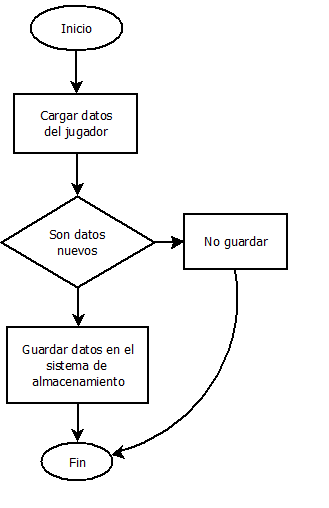
\includegraphics[width=0.5\textwidth]{recursos/Imagenes/DiagramaDatos.png} 
    \caption{Diagrama de Actividades del manejo de guardado de datos}
    \label{fig:mi_imagen}
\end{figure}
\subsubsection{Sitema de feedback visual y sonoro}
\begin{figure}[H]
    \centering
    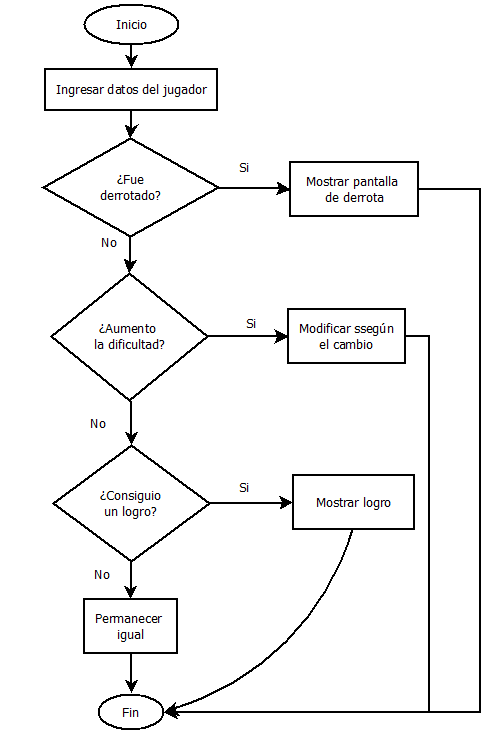
\includegraphics[width=0.5\textwidth]{recursos/Imagenes/DiagramaRetroalimentacion.png} 
    \caption{Diagrama de Actividades del sistema de feedback visual y sonoro}
    \label{fig:mi_imagen}
\end{figure}
    \subsection{Diccionario de Datos}

\subsubsection{Entidad: Jugador}
Esta entidad representa a los jugadores en el sistema, almacenando información básica sobre su identidad y desempeño en el juego.
\begin{table}[H]
\centering
\begin{tabular}{|c|c|c|}
\hline
\textbf{Atributo} & \textbf{Tipo de Dato} & \textbf{Descripción} \\ \hline
J\_ID & \texttt{int} & Identificador único del jugador \\ \hline
Nombre & \texttt{varchar} & Nombre del jugador \\ \hline
Precision & \texttt{float} & Precisión del jugador durante la partida \\ \hline
\end{tabular}
\caption{Entidad Jugador}
\end{table}

\subsubsection{Entidad: Partida}
Esta entidad representa una sesión individual de juego, almacenando datos específicos de cada partida jugada.
\begin{table}[H]
\centering
\begin{tabular}{|c|c|c|}
\hline
\textbf{Atributo} & \textbf{Tipo de Dato} & \textbf{Descripción} \\ \hline
ID & \texttt{int} & Identificador único de la partida \\ \hline
Pje\_P & \texttt{int} & Puntaje obtenido en la partida \\ \hline
HP\_Lost & \texttt{int} & Total de vidas perdidas durante la partida \\ \hline
T\_Jgd & \texttt{float} & Tiempo jugado en minutos \\ \hline
\end{tabular}
\caption{Entidad Partida}
\end{table}

\subsubsection{Entidad: Nivel}
Esta entidad define las características de cada nivel dentro del juego, como su dificultad, enemigos y obstáculos generados.
\begin{table}[H]
\centering
\begin{tabular}{|c|c|c|}
\hline
\textbf{Atributo} & \textbf{Tipo de Dato} & \textbf{Descripción} \\ \hline
ID & \texttt{int} & Identificador único del nivel \\ \hline
Pts\_Obt & \texttt{int} & Puntos obtenidos en el nivel \\ \hline
E\_Gen & \texttt{int} & Enemigos generados en el nivel \\ \hline
E\_Del & \texttt{int} & Enemigos eliminados en el nivel \\ \hline
Obs\_Gen & \texttt{int} & Obstáculos generados en el nivel \\ \hline
N\_Difi & \texttt{int} & Dificultad del nivel \\ \hline
Vel\_Scroll & \texttt{float} & Velocidad de desplazamiento del nivel \\ \hline
\end{tabular}
\caption{Entidad Nivel}
\end{table}

\subsubsection{Entidad: Enemigo}
Esta entidad describe los enemigos que aparecen en el juego, incluyendo su tipo y cantidad de vida.
\begin{table}[H]
\centering
\begin{tabular}{|c|c|c|}
\hline
\textbf{Atributo} & \textbf{Tipo de Dato} & \textbf{Descripción} \\ \hline
ID & \texttt{int} & Identificador único del enemigo \\ \hline
T\_En & \texttt{varchar} & Tipo de enemigo \\ \hline
E\_Enmy & \texttt{int} & Vida del enemigo \\ \hline
\end{tabular}
\caption{Entidad Enemigo}
\end{table}

\subsubsection{Entidad: Ataque}
Esta entidad almacena los datos relativos a los ataques en el juego, como el patrón, frecuencia y potencia del ataque.
\begin{table}[H]
\centering
\begin{tabular}{|c|c|c|}
\hline
\textbf{Atributo} & \textbf{Tipo de Dato} & \textbf{Descripción} \\ \hline
ID & \texttt{int} & Identificador único del ataque \\ \hline
Ptn\_Atq & \texttt{json} & Patrón de ataque \\ \hline
Freq\_Atq & \texttt{int} & Frecuencia de ataque \\ \hline
Pow\_Atq & \texttt{int} & Potencia del ataque \\ \hline
\end{tabular}
\caption{Entidad Ataque}
\end{table}

\subsubsection{Entidad: IA\_Modelo}
Esta entidad contiene los datos relacionados con el modelo de inteligencia artificial utilizado para ajustar la dificultad del juego.
\begin{table}[H]
\centering
\begin{tabular}{|c|c|c|}
\hline
\textbf{Atributo} & \textbf{Tipo de Dato} & \textbf{Descripción} \\ \hline
ID & \texttt{int} & Identificador único del modelo de IA \\ \hline
Metricas & \texttt{json} & Métricas utilizadas por el modelo de IA \\ \hline
Tasa\_Ajst & \texttt{float} & Tasa de ajuste de dificultad \\ \hline
Tm\_Adapt & \texttt{float} & Tiempo de adaptación del modelo \\ \hline
DesvEst & \texttt{float} & Desviación estándar de la dificultad \\ \hline
Heuristica & \texttt{json} & Datos heurísticos utilizados por la IA \\ \hline
\end{tabular}
\caption{Entidad Modelo IA}
\end{table}

\subsubsection{Entidad: Estadísticas}
Esta entidad almacena estadísticas globales y específicas del jugador, como puntajes y precisión, para el análisis del rendimiento.
\begin{table}[H]
\centering
\begin{tabular}{|c|c|c|}
\hline
\textbf{Atributo} & \textbf{Tipo de Dato} & \textbf{Descripción} \\ \hline
ID & \texttt{int} & Identificador único de las estadísticas \\ \hline
M\_Sc & \texttt{int} & Mejor puntaje alcanzado \\ \hline
Ptj\_Ptj & \texttt{int} & Puntaje obtenido en la partida \\ \hline
Best\_Ptj & \texttt{int} & Mejor puntaje registrado \\ \hline
Ttl\_Tiempo & \texttt{float} & Tiempo total jugado \\ \hline
Tm\_media & \texttt{float} & Tiempo medio por partida \\ \hline
PrecisionJdr & \texttt{float} & Precisión promedio del jugador \\ \hline
EstrategiaMov & \texttt{json} & Estrategia de movimiento utilizada por el jugador \\ \hline
\end{tabular}
\caption{Entidad Estadísticas}
\end{table}

\subsection{Relaciones}

\subsubsection{Relación: Juega}
Representa la relación entre un jugador y las partidas que ha jugado. Un jugador puede jugar varias partidas.
\begin{table}[H]
\centering
\begin{tabular}{|c|c|c|}
\hline
\textbf{Entidad 1} & \textbf{Entidad 2} & \textbf{Cardinalidad} \\ \hline
Jugador & Partida & 1:N \\ \hline
\end{tabular}
\caption{Relación Juega entre Jugador y Partida}
\end{table}

\subsubsection{Relación: Posee}
Define la relación entre una partida y los niveles jugados. Una partida puede tener varios niveles.
\begin{table}[H]
\centering
\begin{tabular}{|c|c|c|}
\hline
\textbf{Entidad 1} & \textbf{Entidad 2} & \textbf{Cardinalidad} \\ \hline
Partida & Nivel & 1:N \\ \hline
\end{tabular}
\caption{Relación Posee entre Partida y Nivel}
\end{table}

\subsubsection{Relación: Dispara}
Representa la relación entre un jugador o un enemigo y los ataques que realizan. Un jugador o enemigo puede realizar varios ataques, y un ataque puede ser utilizado por varios enemigos.
\begin{table}[H]
\centering
\begin{tabular}{|c|c|c|}
\hline
\textbf{Entidad 1} & \textbf{Entidad 2} & \textbf{Cardinalidad} \\ \hline
Jugador & Ataque & 1:N \\ \hline
Enemigo & Ataque & N:M \\ \hline
\end{tabular}
\caption{Relación Dispara entre Jugador/Enemigo y Ataque}
\end{table}

\subsubsection{Relación: Modifica}
Define la relación entre el modelo de IA y los enemigos, indicando que el modelo de IA puede modificar varios enemigos, y un enemigo puede ser modificado por varios modelos de IA.
\begin{table}[H]
\centering
\begin{tabular}{|c|c|c|}
\hline
\textbf{Entidad 1} & \textbf{Entidad 2} & \textbf{Cardinalidad} \\ \hline
IA\_Modelo & Enemigo & 1:N \\ \hline
\end{tabular}
\caption{Relación Modifica entre IA\_Modelo y Enemigo}
\end{table}

\subsubsection{Relación: Genera}
Representa la relación entre la IA y las estadísticas generadas a partir del comportamiento de los jugadores. El modelo de IA puede generar varias estadísticas.
\begin{table}[H]
\centering
\begin{tabular}{|c|c|c|}
\hline
\textbf{Entidad 1} & \textbf{Entidad 2} & \textbf{Cardinalidad} \\ \hline
IA\_Modelo & Estadísticas & 1:N \\ \hline
\end{tabular}
\caption{Relación Genera entre IA\_Modelo y Estadísticas}
\end{table}

    \subsection{Diagrama Entidad-Relación (E-R)}
\begin{figure}[H]
\centering
\begin{adjustbox}{width=\textwidth} % Ajusta el diagrama al ancho de la página
\begin{tikzpicture}
\begin{dot2tex}[styleonly, mathmode, codeonly, neato, options=-s]
digraph G {
    // Ajustes generales del grafo
    graph [rankdir=LR, ranksep=15, nodesep=15];  // Cambia a LR para dirección horizontal

    // Estilo de las conexiones
    edge [style="simple relation"];
    
    // Estilos personalizados
    node [style="rounded", fontsize=12, shape=rectangle, width=2.5]; // Cambia el tamaño de los nodos
    
    // Entidades
    Jugador [style="entity", label="Jugador"];
    Jid [style="attribute", label="\underline{J\_ID}"];
    Nombre [style="attribute", label="Name"];
    
    Partida [style="entity", label="Partida"];
    Pid [style="attribute", label="\underline{ID}"];
    PuntajePartida [style="attribute", label="Pje_P"];
    vPerd [style="attribute", label="HP\_Lost"];
    tJug [style="attribute", label="T\_Jgd"];

    Nivel [style="entity", label="Nivel"];
    Nid [style="attribute", label="\underline{ID}"];
    pObt [style="attribute", label="Pts\_Obt"];
    eGen [style="attribute", label="E\_Gen"];
    eElim [style="derived attribute", label="E\_Del"];
    oGen [style="attribute", label="Obs\_Gen"];
    dNiv [style="attribute", label="N\_Difi"];
    VelScroll [style="attribute", label="Vel\_Scroll"]; // Corregido "Sreoll"

    Enemigo [style="entity", label="Enemigos"];
    Eid [style="attribute", label="\underline{ID}"];
    Tipo [style="attribute", label="T\_En"];
    vEnm [style="attribute", label="E\_Enmy"];

    Ataque [style="weak entity"];
    IdAtq [style="attribute", label="\dashedunderline{ID}"];
    PtnAtq [style="multi attribute", label="Ptn\_Atq"];
    FreqAtq [style="attribute", label="Freq\_Atq"];
    PowAtq [style="attribute", label="Pow\_Atq"];
    
    IA_Modelo [style="entity", label="Modelo\_IA"];
    Mid [style="attribute", label="\underline{ID}"];
    Metricas [style="attribute", label="Metricas"]; //Añadido label
    TasaAjuste [style="attribute", label="Tasa\_Ajst"];
    TiempoAdpt [style="attribute", label="Tm\_Adapt"];
    DestEstDif [style="attribute", label="DesvEst"];
    Heuristica [style="attribute", label="Heuristica"];
    
    Estadisticas [style="weak entity"];
    idEstad [style="attribute", label="\dashedunderline{ID}"];
    MScore [style="attribute", label="M\_Sc"];
    PuntajePartida [style="attribute", label="Ptj\_Ptj"];
    MejorPuntaje [style="attribute", label="Best\_Ptj"];
    TtlTiempo [style="attribute", label="Ttl\_Tiempo"];
    TiempoMedio [style="attribute", label="Tm\_media"];
    PresicionJdr [style="attribute", label="PrecisionJdr"];
    estrategiaMov [style="attribute", label="EstrategiaMov"];
    
    // Relaciones
    juega [style="relationship"];
    posee [style="relationship"];
    TtlEnDel [style="derived attribute"];
    tiene [style="relationship"];
    disparaJdr [style="weak relationship", label="dispara"];
    disparaEne [style="weak relationship", label="dispara"];
    modifica [style="relationship"];
    cambia [style="relationship"];
    transforma [style="relationship"];
            
    genera [style="weak relationship"];
    usa [style="weak relationship"];
    
    // Conexiones
    Jugador -> Jid;
    Jugador -> Nombre;
    
    Partida -> Pid;
    Partida -> PuntajePartida;
    Partida -> vPerd;
    Partida -> tJug;
    
    Nivel -> Nid;
    Nivel -> eGen;
    Nivel -> eElim;
    Nivel -> oGen;
    Nivel -> dNiv;
    Nivel -> VelScroll;
    Nivel -> pObt;
    
    Enemigo -> Eid;
    Enemigo -> Tipo;
    Enemigo -> vEnm;

    Ataque -> IdAtq;
    Ataque -> PtnAtq;
    Ataque -> FreqAtq;
    Ataque -> PowAtq;

    Estadisticas -> idEstad;
    Estadisticas -> MScore;
    Estadisticas -> PuntajePartida;
    Estadisticas -> MejorPuntaje;
    Estadisticas -> TtlTiempo; 
    Estadisticas -> TiempoMedio; 
    Estadisticas -> PresicionJdr; 
    Estadisticas -> estrategiaMov; 
    
    IA_Modelo -> Mid;
    IA_Modelo -> Metricas;
    IA_Modelo -> Metricas -> TasaAjuste;
    IA_Modelo -> Metricas -> TiempoAdpt;
    IA_Modelo -> Metricas -> DestEstDif;
    IA_Modelo -> Heuristica;

    // Relaciones
    Jugador -> juega [label="1"];
    Partida -> juega [style="total relation", label="N"];
    
    Partida -> posee [style="total relation", label="1"];
    Nivel -> posee [style="total relation", label="N"];
    posee -> TtlEnDel;
    
    Enemigo -> tiene [label="M"];
    Nivel -> tiene [style="total relation", label="N"];

    Jugador -> disparaJdr [style="total relation", label="1"];
    Ataque -> disparaJdr [label="1"];

    Enemigo -> disparaEne [style="total relation", label="N"];
    Ataque -> disparaEne [label="M"];

    IA_Modelo -> modifica [style="total relation", label="N"];
    Enemigo -> modifica [label="M"];

    IA_Modelo -> cambia [style="total relation", label="N"];
    Nivel -> cambia [label="M"];

    Jugador -> genera [label="1"];
    IA_Modelo -> genera [style="total relation", label="M"];

    Partida -> usa [label="N"]; // Corregido "Usa" -> "usa"
    IA_Modelo -> usa [label="1"];

    Estadisticas -> transforma [label="N"];
    IA_Modelo -> transforma [label="1"];
}
\end{dot2tex}
\end{tikzpicture}
\end{adjustbox}
\caption{Diagrama de entidad-relación de ejemplo}
\label{fig:diagrama_ER}
\end{figure}

    \subsection*{Diagramas de vistas.}
\subsection{Generación Procedural de Niveles}
\subsubsection{Vista  Funcional}
Este diagrama representa la Vista de Caso de Uso para la Generación Procedural de Niveles. Describe las interacciones entre los actores principales del sistema y el proceso de generación de niveles.
\begin{figure}[H]
\centering
\begin{adjustbox}{width=0.45\textwidth}
\begin{tikzpicture}[
    process/.style={rectangle, draw, minimum height=1cm, minimum width=3.5cm, align=center},
    entity/.style={ellipse, draw, minimum height=1cm, minimum width=2.5cm, align=center},
    relation/.style={-Stealth, thick}
]

% Entities
\node[entity] (jugador) {Jugador};
\node[entity, below=of jugador] (partida) {Partida};
\node[entity, right=of partida] (nivel) {Nivel};
\node[entity, below=of partida] (enemigo) {Enemigo};
\node[entity, right=of enemigo] (ataque) {Ataque};

% Processes
\node[process, right=of jugador, xshift=3cm] (vars) {Recepción de Variables de Dificultad};
\node[process, below=of vars] (enemigoSel) {Selección de Enemigos};
\node[process, below=of enemigoSel] (patronGen) {Generación de Patrones de Ataque};
\node[process, below=of patronGen] (ajuste) {Ajuste Procedural de Patrones};
\node[process, below=of ajuste] (verif) {Verificación de Reglas de Juego};
\node[process, below=of verif] (implement) {Implementación de Enemigos en el Nivel};

% Arrows between processes
\draw[relation] (vars) -- (enemigoSel);
\draw[relation] (enemigoSel) -- (patronGen);
\draw[relation] (patronGen) -- (ajuste);
\draw[relation] (ajuste) -- (verif);
\draw[relation] (verif) -- (implement);

% Arrows between entities and processes
\draw[relation] (jugador) -- (vars);
\draw[relation] (nivel) -- (enemigoSel);
\draw[relation] (enemigo) -- (enemigoSel);
\draw[relation] (ataque) -- (patronGen);

% Relationships
\draw[relation, dashed] (jugador) -- (partida) node[midway, right] {Juega};
\draw[relation, dashed] (partida) -- (nivel) node[midway, below] {Posee};
\draw[relation, dashed] (enemigo) -- (ataque) node[midway, below] {Dispara};

\end{tikzpicture}
\end{adjustbox}
\caption{Vista Funcional}
\end{figure}

\subsubsection{Vista  Lógica}
Este diagrama representa la Vista Lógica (Diagrama de Clases) para el sistema de generación procedural de niveles, mostrando las principales clases y sus interacciones. A su ves proporciona una visión clara de cómo las distintas clases y componentes del sistema interactúan entre sí en el contexto de la generación procedural de niveles.
\begin{figure}[H]
\centering
\begin{adjustbox}{width=0.6\textwidth}
\begin{tikzpicture}[
    class/.style={rectangle, draw, minimum width=3cm, minimum height=1.5cm, align=center},
    relationship/.style={-Stealth, thick}
]

% Classes
\node[class] (nivel) {Nivel\\
\textbf{Atributos:}\\
ID\\
Puntos Obtenidos\\
Enemigos Generados\\
Dificultad};

\node[class, below=of nivel] (motor_procedural) {MotorProcedural\\
\textbf{Atributos:}\\
Obstáculos Generados\\
Vel\_Scroll};

\node[class, right=of nivel, xshift=3cm] (sistema_ia) {SistemaIA\\
\textbf{Atributos:}\\
Métricas\\
Tasa\_Ajst\\
Tiempo de Adaptación};

\node[class, below=of motor_procedural] (jugador) {Jugador\\
\textbf{Atributos:}\\
J\_ID\\
Nombre\\
Precisión};

% Relationships
\draw[relationship] (nivel) -- (motor_procedural) node[midway, right] {depende de};
\draw[relationship] (nivel) -- (sistema_ia) node[midway, above] {interactúa con};
\draw[relationship] (jugador) -- (sistema_ia) node[midway, right] {influye en};
\draw[relationship] (jugador) -- (motor_procedural) node[midway, right] {influye en};

\end{tikzpicture}
\end{adjustbox}
\caption{Vista Lógica}
\end{figure}

\subsubsection{Vista  de Secuencia}
Este Diagrama de Secuencia muestra la interacción y el flujo de mensajes entre los actores principales y los componentes del sistema durante la generación de un nivel procedimental. Además de mostrar cómo las interacciones temporales entre los componentes del sistema aseguran que el nivel generado sea jugable y esté ajustado adecuadamente en cuanto a dificultad y distribución de enemigos.
\begin{figure}[H]
\centering
\begin{adjustbox}{width=0.6\textwidth}

\begin{tikzpicture}[
    actor/.style={rectangle, draw, text centered, minimum width=2.5cm, minimum height=1cm},
    message/.style={->, thick, >=Stealth},
    every node/.style={align=center}
]

% Actors
\node (jugador) [actor] {Jugador};
\node (ia) [actor, right=3cm of jugador] {Sistema de IA};
\node (procedural) [actor, right=3cm of ia] {Motor Procedural};
\node (nivel) [actor, right=3cm of procedural] {Nivel};

% Messages
\draw[message] (jugador) -- node[above] {Inicia Partida} (ia);
\draw[message] (ia) -- node[above] {Recibe Parámetros} (procedural);
\draw[message] (procedural) -- node[above] {Genera Entorno} (nivel);
\draw[message] (ia) -- +(0,-1.5) -| node[below] {Distribuye Enemigos \\ Ajusta Dificultad} (nivel);
\draw[message] (nivel) -- node[below] {Verifica Reglas} (ia);
\draw[message] (nivel) -- node[below] {Nivel Listo para Jugar} (jugador);

\end{tikzpicture}
\end{adjustbox}
\caption{Vista de Secuencia}
\end{figure}

\subsubsection{Vista  de Despliegue}
Este diagrama asegura que los roles y responsabilidades de los componentes estén claramente separados, con el servidor encargado de la lógica pesada y el cliente enfocado en la interacción con el jugador.
\begin{figure}[H]
\centering
\begin{adjustbox}{width=0.6\textwidth}
\begin{tikzpicture}[
    server/.style={rectangle, draw, text centered, minimum width=4cm, minimum height=1cm, fill=blue!20},
    client/.style={rectangle, draw, text centered, minimum width=4cm, minimum height=1cm, fill=green!20},
    connection/.style={->, thick, >=Stealth}
]

% Components
\node (server) [server] {Servidor del Juego\\(Motor Procedural, Sistema de IA)};
\node (client) [client, below=2cm of server] {Cliente (Jugador)\\(Dispositivo del Jugador)};

% Entities on server
\node (nivel) [right=0.5cm of server, align=center] {Entidad Nivel};
\node (ia_modelo) [right=0.5cm of nivel, align=center] {Entidad IA\\Modelo};

% Entities on client
\node (jugador) [right=0.5cm of client, align=center] {Entidad Jugador};

% Connections
\draw[connection] (client) -- node[midway, right] {Interacción con el sistema} (server);
\draw[connection] (server) -- (nivel);
\draw[connection] (server) -- (ia_modelo);
\draw[connection] (client) -- (jugador);

\end{tikzpicture}
\end{adjustbox}
\caption{Vista de Despliegue}
\end{figure}

\subsubsection{Vista  de Estados}
Este Diagrama de Estados muestra los estados por los que pasa un nivel durante su generación procedural en el sistema.
\begin{figure}[H]
\centering
\begin{adjustbox}{width=0.5\textwidth}
\begin{tikzpicture}[
    ->, >=Stealth, 
    node distance=2cm, 
    state/.style={rectangle, draw, minimum width=3cm, align=center, rounded corners}
]

% States
\node[state] (esperando) {EsperandoInicio\\(Entidad Jugador)};
\node[state] (generando) [below=of esperando] {GenerandoEntorno\\(Entidad Nivel)};
\node[state] (obstaculos) [below=of generando] {DistribuyendoObstáculos\\(Entidad Nivel)};
\node[state] (enemigos) [below=of obstaculos] {DistribuyendoEnemigos\\(Entidad Enemigo)};
\node[state] (verificando) [below=of enemigos] {VerificandoReglas\\(Entidad Nivel)};
\node[state] (listo) [below=of verificando] {NivelListo\\(Entidad Nivel)};

% Transitions
\draw (esperando) edge[bend left] node[right] {Iniciar Partida} (generando);
\draw (generando) edge[bend left] node[right] {Entorno Generado} (obstaculos);
\draw (obstaculos) edge[bend left] node[right] {Obstáculos Colocados} (enemigos);
\draw (enemigos) edge[bend left] node[right] {Enemigos Posicionados} (verificando);
\draw (verificando) edge[bend left] node[right] {Reglas Validadas} (listo);

\end{tikzpicture}
\end{adjustbox}
\caption{Vista de Estados}
\end{figure}

\subsection{Entrenamiento de IA}
\subsubsection{Vista Lógica}

\begin{figure}[H]
\centering
\begin{adjustbox}{width=\textwidth}
\begin{tikzpicture}[
    component/.style={rectangle, draw, minimum height=1cm, minimum width=2.5cm, align=center}
]

\node[component] (ia) {Motor de IA};
\node[component, above=of ia] (preproc) {Módulo de Preprocesamiento};
\node[component, below=of ia] (rednn) {Red Neuronal};
\node[component, left=of ia] (eval) {Módulo de Evaluación};
\node[component, right=of ia] (param) {Módulo de Ajuste de\\Parámetros};

% Arrows between components
\draw (preproc) -> (ia);
\draw (ia) -> (rednn);
\draw (eval) -> (ia);
\draw (param) -> (ia);

\end{tikzpicture}
\end{adjustbox}
\caption{Vista Lógica del Sistema}
\end{figure}

\subsubsection{Vista de Infraestructura}
\begin{figure}[H]
\centering
\begin{adjustbox}{width=\textwidth}
\begin{tikzpicture}[
    server/.style={rectangle, draw, minimum height=1cm, minimum width=2.5cm, align=center}
]

\node[server] (data) {Servidor de Datos};
\node[server, right=of data] (train) {Servidor de IA/Entrenamiento};
\node[server, right=of train] (client) {Cliente del Juego};

% Arrows between servers
\draw (data) -> (train);
\draw (train) -> (client);

\end{tikzpicture}
\end{adjustbox}
\caption{Vista de Infraestructura del proceso}
\end{figure}

\subsubsection{Vista de Desarrollo}
\begin{figure}[H]
\centering
\begin{adjustbox}{width=0.8\textwidth}
\begin{tikzpicture}[
    class/.style={rectangle, draw, minimum height=1cm, minimum width=3cm, align=center}
]

\node[class] (data) {Recoleccion de datos};
\node[class, below=of data] (preproc) {Pre-procesamiento};
\node[class, below=of preproc] (trainer) {Modulo de\\Entrenamiento};
\node[class, right=of trainer] (eval) {Modulo de\\Evaluación};
\node[class, left=of trainer] (adjust) {Ajustador de\\Parámetros};

% Arrows between classes
\draw (data) -> (preproc);
\draw (preproc) -> (trainer);
\draw (trainer) -> (eval);
\draw (adjust) -> (trainer);

\end{tikzpicture}
\end{adjustbox}
\caption{Vista de Desarrollo}
\end{figure}

\subsubsection{Vista de Ejecucion}
\begin{figure}[H]
\centering
\begin{adjustbox}{width=0.5\textwidth}

\begin{tikzpicture}[
    server/.style={rectangle, draw, minimum height=1cm, minimum width=3.5cm, align=center}
]

\node[server] (rec) {Recopilación de Datos};
\node[server, below=of rec] (preproc) {Preprocesamiento};
\node[server, below=of preproc] (train) {Entrenamiento de IA};
\node[server, below=of train] (eval) {Evaluación del Modelo};
\node[server, below=of eval] (adjust) {Ajuste de Parámetros};
\node[server, below=of adjust] (deploy) {Implementación del Modelo};

% Arrows between servers
\draw (rec) -> (preproc);
\draw (preproc) -> (train);
\draw (train) -> (eval);
\draw (eval) -> (adjust);
\draw (adjust) -> (deploy);

\end{tikzpicture}
\end{adjustbox}
\caption{Vista de Ejecucion}
\end{figure}

\subsubsection{Vista Funcional}
\begin{figure}[H]
\centering
\begin{adjustbox}{width=0.5\textwidth}
\begin{tikzpicture}[
    actor/.style={circle, draw, minimum height=1cm, align=center},
    case/.style={rectangle, draw, minimum height=1cm, minimum width=3cm, align=center}
]

\node[actor] (player) {Jugador};
\node[case, right=of player] (train) {Entrenar IA};
\node[case, below=of train] (eval) {Evaluar IA};
\node[case, below=of eval] (adjust) {Ajustar IA};

% Arrows between actor and use cases
\draw (player) -> (train);
\draw (train) -> (eval);
\draw (eval) -> (adjust);

\end{tikzpicture}
\end{adjustbox}
\caption{Vista Funcional}
\end{figure}


\subsection{Gestión de Enemigos y Patrones de Ataque}
\subsubsection{Vista  Funcional}
Este diagrama muestra cómo las entidades y procesos interactúan para gestionar la dificultad y ajustar los patrones de ataque de los enemigos en tiempo real, de acuerdo con el progreso del jugador.
\begin{figure}[H]
\centering
\begin{adjustbox}{width=0.6\textwidth}
\begin{tikzpicture}[
    process/.style={rectangle, draw, minimum height=1cm, minimum width=3.5cm, align=center},
    entity/.style={ellipse, draw, minimum height=1cm, minimum width=2.5cm, align=center},
    relation/.style={-Stealth, thick}
]

% Entities
\node[entity] (jugador) {Jugador};
\node[entity, below=of jugador] (partida) {Partida};
\node[entity, right=of partida] (nivel) {Nivel};
\node[entity, below=of partida] (enemigo) {Enemigo};
\node[entity, right=of enemigo] (ataque) {Ataque};

% Processes
\node[process, right=of jugador, xshift=3cm] (vars) {Recepción de Variables de Dificultad};
\node[process, below=of vars] (enemigoSel) {Selección de Enemigos};
\node[process, below=of enemigoSel] (patronGen) {Generación de Patrones de Ataque};
\node[process, below=of patronGen] (ajuste) {Ajuste Procedural de Patrones};
\node[process, below=of ajuste] (verif) {Verificación de Reglas de Juego};
\node[process, below=of verif] (implement) {Implementación de Enemigos en el Nivel};

% Arrows between processes
\draw[relation] (vars) -- (enemigoSel);
\draw[relation] (enemigoSel) -- (patronGen);
\draw[relation] (patronGen) -- (ajuste);
\draw[relation] (ajuste) -- (verif);
\draw[relation] (verif) -- (implement);

% Arrows between entities and processes
\draw[relation] (jugador) -- (vars);
\draw[relation] (nivel) -- (enemigoSel);
\draw[relation] (enemigo) -- (enemigoSel);
\draw[relation] (ataque) -- (patronGen);

% Relationships
\draw[relation, dashed] (jugador) -- (partida) node[midway, right] {Juega};
\draw[relation, dashed] (partida) -- (nivel) node[midway, below] {Posee};
\draw[relation, dashed] (enemigo) -- (ataque) node[midway, below] {Dispara};

\end{tikzpicture}
\end{adjustbox}
\caption{Vista Funcional}
\end{figure}

\subsubsection{Vista  de Comportamientos}
Este diagrama destaca cómo el sistema de IA responde al rendimiento del jugador y ajusta dinámicamente tanto los enemigos como los patrones de ataque para mantener la jugabilidad equilibrada.
\begin{figure}[H]
\centering
\begin{adjustbox}{width=0.75\textwidth}
\begin{tikzpicture}[
    process/.style={rectangle, draw, minimum height=1cm, minimum width=4cm, align=center},
    entity/.style={ellipse, draw, minimum height=1cm, minimum width=2.5cm, align=center},
    relation/.style={-Stealth, thick}
]

% Entities
\node[entity] (jugador) {Jugador};
\node[entity, right=of jugador, xshift=3cm] (ia) {IA\_Modelo};
\node[entity, below=of ia] (enemigo) {Enemigo};
\node[entity, below=of enemigo] (ataque) {Ataque};

% Processes
\node[process, below=of jugador] (analisis) {Análisis del Rendimiento del Jugador};
\node[process, below=of analisis] (ajusteDificultad) {Ajuste de Dificultad};
\node[process, below=of ajusteDificultad] (ajustePatrones) {Ajuste Procedural de Patrones de Ataque};

% Arrows between processes
\draw[relation] (analisis) -- (ajusteDificultad);
\draw[relation] (ajusteDificultad) -- (ajustePatrones);

% Arrows between entities and processes
\draw[relation] (jugador) -- (analisis);
\draw[relation] (ia) -- (ajusteDificultad);
\draw[relation] (ia) -- (ajustePatrones);
\draw[relation] (ajusteDificultad) -- (enemigo);
\draw[relation] (ajustePatrones) -- (ataque);

% Relationships
\draw[relation, dashed] (ia) -- (enemigo) node[midway, right] {Modifica};
\draw[relation, dashed] (enemigo) -- (ataque) node[midway, right] {Dispara};

\end{tikzpicture}
\end{adjustbox}
\caption{Vista de Comportamientos}
\end{figure}

\subsubsection{Vista  de Infraestructura}
Este diagrama representa cómo se distribuye el sistema en la infraestructura y cómo interactúan los componentes físicos.
\begin{figure}[H]
\centering
\begin{adjustbox}{width=0.95\textwidth}
\begin{tikzpicture}[
    server/.style={cylinder, shape border rotate=90, draw, minimum height=2cm, minimum width=1cm, cylinder uses custom fill, cylinder body fill=blue!30, cylinder end fill=blue!10, align=center},
    process/.style={rectangle, draw, minimum height=1cm, minimum width=3cm, align=center},
    entity/.style={ellipse, draw, minimum height=1cm, minimum width=2.5cm, align=center},
    relation/.style={-Stealth, thick},
    client/.style={rectangle, draw, rounded corners, minimum height=1cm, minimum width=3cm, align=center, fill=green!20}
]

% Entities
\node[client] (clienteJuego) {Cliente del Juego};
\node[server, right=of clienteJuego, xshift=3cm] (servidorIA) {Servidor de IA/Entrenamiento};
\node[server, right=of servidorIA, xshift=3cm] (servidorDatos) {Servidores de Datos};

% Almacenamiento de Datos Históricos above Data Server
\node[process, above=of servidorDatos, yshift=1cm] (almacenamiento) {Almacenamiento de Datos Históricos};

% Components on client
\node[process, below=of clienteJuego] (iaModelo) {IA\_Modelo};
\node[process, below=of iaModelo] (nivel) {Nivel};
\node[process, below=of nivel] (enemigo) {Enemigo};

% Components on IA server
\node[entity, below=of servidorIA] (estadisticas) {Estadísticas};

% Arrows between client components
\draw[relation] (clienteJuego) -- (iaModelo);
\draw[relation] (iaModelo) -- (nivel);
\draw[relation] (nivel) -- (enemigo);

% Arrows between servers and client
\draw[relation] (servidorIA) -- (iaModelo) node[midway, above] {Modelo Entrenado};
\draw[relation] (servidorIA) -- (estadisticas) node[midway, right] {Genera};
\draw[relation] (servidorDatos) -- (servidorIA) node[midway, above] {Datos Preprocesados};

% Arrows between data server and IA server
\draw[relation] (almacenamiento) -- (servidorDatos) node[midway, right] {Datos Históricos};

% Relationships
\draw[relation, dashed] (iaModelo) -- (enemigo) node[midway, right] {Modifica};
\draw[relation, dashed] (estadisticas) -- (servidorDatos) node[midway, right] {Almacena};
\draw[relation, dashed] (estadisticas) -- (iaModelo) node[midway, left] {Genera};

\end{tikzpicture}

\end{adjustbox}
\caption{Vista de Infraestructura}
\end{figure}

\subsubsection{Vista  de Ejecución}
Este diagrama muestra los pasos que sigue el sistema para el entrenamiento del modelo de IA, centrado en el flujo de trabajo y la interacción entre las diferentes entidades involucradas.
\begin{figure}[H]
\centering
\begin{adjustbox}{width=0.75\textwidth}
\begin{tikzpicture}[
    process/.style={rectangle, draw, minimum height=1cm, minimum width=3cm, align=center, rounded corners},
    entity/.style={ellipse, draw, minimum height=1cm, minimum width=2.5cm, align=center},
    relation/.style={-Stealth, thick}
]

% Nodes (Steps in the process)
\node[process] (recopilacion) {Recopilación de Datos Históricos};
\node[process, below=of recopilacion] (preprocesamiento) {Preprocesamiento de Datos};
\node[process, below=of preprocesamiento] (entrenamiento) {Entrenamiento de la IA};
\node[process, below=of entrenamiento] (evaluacion) {Evaluación del Modelo};
\node[process, below=of evaluacion] (ajuste) {Ajuste de Parámetros};
\node[process, below=of ajuste] (implementacion) {Implementación del Modelo};

% Entities
\node[entity, left=of preprocesamiento, xshift=-2cm] (nivel) {Nivel};
\node[entity, right=of preprocesamiento, xshift=2cm] (partida) {Partida};
\node[entity, left=of entrenamiento, xshift=-2cm] (jugador) {Jugador};
\node[entity, right=of evaluacion, xshift=2cm] (estadisticas) {Estadísticas};
\node[entity, left=of implementacion, xshift=-2cm] (ia_modelo) {IA\_Modelo};

% Relations between steps (process flow)
\draw[relation] (recopilacion) -- (preprocesamiento);
\draw[relation] (preprocesamiento) -- (entrenamiento);
\draw[relation] (entrenamiento) -- (evaluacion);
\draw[relation] (evaluacion) -- (ajuste);
\draw[relation] (ajuste) -- (implementacion);

% Relationships to entities
\draw[relation, dashed] (nivel) -- (preprocesamiento);
\draw[relation, dashed] (partida) -- (preprocesamiento);
\draw[relation, dashed] (jugador) -- (entrenamiento);
\draw[relation, dashed] (estadisticas) -- (evaluacion);
\draw[relation, dashed] (ia_modelo) -- (implementacion);

\end{tikzpicture}
\end{adjustbox}
\caption{Vista de Ejecución}
\end{figure}

\subsubsection{Vista  de Integración}
Este diagrama muestra cómo el proceso de Gestión de Enemigos y Patrones de Ataque se integra con otros procesos importantes dentro del sistema para garantizar una experiencia de juego cohesiva y adaptativa.
\begin{figure}[H]
\centering
\begin{adjustbox}{width=\textwidth}
\begin{tikzpicture}[
    process/.style={rectangle, draw, minimum height=1cm, minimum width=3cm, align=center, rounded corners},
    entity/.style={ellipse, draw, minimum height=1cm, minimum width=2.5cm, align=center},
    relation/.style={-Stealth, thick}
]

% Nodes (Processes)
\node[process] (gestion) {Gestión de Enemigos y Patrones de Ataque};
\node[process, above left=of gestion, xshift=-1cm, yshift=2cm] (generacion) {Generación Procedural de Niveles};
\node[process, above right=of gestion, xshift=1cm, yshift=2cm] (ajuste) {Ajuste Dinámico de Dificultad};
\node[process, below=of gestion, yshift=-2cm] (interfaz) {Interfaz de Usuario};

% Entities
\node[entity, below left=of gestion, xshift=-1cm] (nivel) {Nivel};
\node[entity, below right=of gestion, xshift=1cm] (partida) {Partida};
\node[entity, below=of interfaz, yshift=-1cm] (jugador) {Jugador};
\node[entity, below=of partida, yshift=-1cm] (estadisticas) {Estadísticas};
\node[entity, right=of ajuste, xshift=2cm] (ia_modelo) {IA\_Modelo};

% Relations between processes
\draw[relation] (generacion) -- (gestion);
\draw[relation] (ajuste) -- (gestion);
\draw[relation] (gestion) -- (interfaz);

% Relations to entities
\draw[relation, dashed] (nivel) -- (gestion);
\draw[relation, dashed] (partida) -- (gestion);
\draw[relation, dashed] (jugador) -- (interfaz);
\draw[relation, dashed] (estadisticas) -- (gestion);
\draw[relation, dashed] (ia_modelo) -- (ajuste);

\end{tikzpicture}
\end{adjustbox}
\caption{Vista de Integración}
\end{figure}

\subsubsection{Vista  de Verificación y Validación}
Este diagrama ilustra el proceso de verificación de las reglas dentro del sistema de juego, para asegurarse de que los patrones de ataque y los enemigos seleccionados sean viables y cumplan con las normas de jugabilidad.
\begin{figure}[H]
\centering
\begin{adjustbox}{width=\textwidth}
\begin{tikzpicture}[
    process/.style={rectangle, draw, minimum height=1cm, minimum width=3cm, align=center, rounded corners},
    entity/.style={ellipse, draw, minimum height=1cm, minimum width=2.5cm, align=center},
    validation/.style={diamond, draw, aspect=2, minimum width=3cm, align=center},
    relation/.style={-Stealth, thick}
]

% Nodes (Processes)
\node[process] (generar) {Generar Patrones de Ataque};
\node[process, below=of generar, yshift=-2cm] (seleccionar) {Seleccionar Enemigos};
\node[validation, right=of generar, xshift=2cm] (verificar) {Verificación de Reglas};

% Entities
\node[entity, left=of generar, xshift=-2cm] (ataque) {Ataque};
\node[entity, below left=of seleccionar, xshift=-1cm, yshift=-1cm] (enemigo) {Enemigo};
\node[entity, below right=of seleccionar, xshift=1cm, yshift=-1cm] (nivel) {Nivel};

% Relations between processes
\draw[relation] (generar) -- (verificar);
\draw[relation] (seleccionar) -- (verificar);

% Relations to entities
\draw[relation, dashed] (ataque) -- (generar);
\draw[relation, dashed] (enemigo) -- (seleccionar);
\draw[relation, dashed] (nivel) -- (verificar);

% Additional Labels
\node[below=of verificar, yshift=-0.5cm, align=center] (validation_note) {Verificación: \\ Patrones viables y respetan reglas del juego};

\end{tikzpicture}
\end{adjustbox}
\caption{Vista de Verificación y Validación}
\end{figure}

\subsubsection{Vista  de Desempeño y Escalabilidad}
Este diagrama representa la Vista de Desempeño o Escalabilidad del sistema, destacando los procesos clave que aseguran un rendimiento adecuado en tiempo real sin afectar la fluidez del juego.
\begin{figure}[H]
\centering
\begin{adjustbox}{width=0.8\textwidth}
\begin{tikzpicture}[
    process/.style={rectangle, draw, minimum height=1cm, minimum width=3cm, align=center, rounded corners},
    entity/.style={ellipse, draw, minimum height=1cm, minimum width=2.5cm, align=center},
    check/.style={diamond, draw, aspect=2, minimum width=3cm, align=center},
    relation/.style={-Stealth, thick}
]

% Nodes (Processes)
\node[process] (ajustar) {Ajuste Procedural en Tiempo Real};
\node[process, below=of ajustar, yshift=-2cm] (verificar) {Verificar Desempeño del Nivel};
\node[process, below=of verificar, yshift=-2cm] (optimizar) {Optimizar Rendimiento del Juego};

% Entities
\node[entity, left=of ajustar, xshift=-2cm] (ia_modelo) {IA\_Modelo};
\node[entity, below left=of verificar, xshift=-1cm, yshift=-1cm] (enemigo) {Enemigo};
\node[entity, below right=of verificar, xshift=1cm, yshift=-1cm] (nivel) {Nivel};

% Relations between processes
\draw[relation] (ajustar) -- (verificar);
\draw[relation] (verificar) -- (optimizar);

% Relations to entities
\draw[relation, dashed] (ia_modelo) -- (ajustar);
\draw[relation, dashed] (enemigo) -- (verificar);
\draw[relation, dashed] (nivel) -- (optimizar);

% Additional Labels
\node[below=of optimizar, yshift=-0.5cm, align=center] (note) {Asegura fluidez \\ incluso con niveles complejos};

\end{tikzpicture}
\end{adjustbox}
\caption{Vista de Desempeño y Escalabilidad}
\end{figure}

\subsection{Registro y análisis de puntuación}
\subsubsection{Diagrama de Vistas de la Optimización del Rendimiento}
\begin{figure}[H]
\centering
\begin{adjustbox}{width=0.6\textwidth}
\begin{tikzpicture}[
    class/.style={rectangle, draw, minimum height=1cm, minimum width=3cm, align=center}
]

% Definir las clases
\node[class] (recursos) {Obtener Recursos\\ del Juego};
\node[class, below=of recursos] (carga) {Monitorear Carga\\ del Sistema};
\node[class, below=of carga] (frame) {Verificar Frame\\ Rate Actual};
\node[class, below=of frame] (ajustar) {Ajustar\\ Rendimiento};
\node[class, below=of ajustar] (optimizar) {Optimizar\\ Rendimiento};

% Conectar las clases
\draw (recursos) -> (carga);
\draw (carga) -> (frame);
\draw (frame) -> (ajustar);
\draw (ajustar) -> (optimizar);

% Añadir decisiones
\node[class, right=of ajustar] (decision) {¿Frame Rate < 60 FPS?};
\draw (ajustar.east) -- (decision);
\draw (decision.east) --++(1,0) node [above] {Sí} |- (optimizar);
\draw (decision.east) --++(1,0) node [below] {No} --++(0,-1) |- (optimizar.east);

\end{tikzpicture}
\end{adjustbox}
\caption{Vista de Desarrollo de la Optimización del Rendimiento}
\end{figure}

\subsection{Optimización de rendimiento}
\subsubsection{Diagrama de Vistas de la Optimización del Rendimiento}
\begin{figure}[H]
\centering
\begin{adjustbox}{width=0.6\textwidth}
\begin{tikzpicture}[
    class/.style={rectangle, draw, minimum height=1cm, minimum width=3cm, align=center}
]

% Definir las clases
\node[class] (recursos) {Obtener Recursos\\ del Juego};
\node[class, below=of recursos] (carga) {Monitorear Carga\\ del Sistema};
\node[class, below=of carga] (frame) {Verificar Frame\\ Rate Actual};
\node[class, below=of frame] (ajustar) {Ajustar\\ Rendimiento};
\node[class, below=of ajustar] (optimizar) {Optimizar\\ Rendimiento};

% Conectar las clases
\draw (recursos) -> (carga);
\draw (carga) -> (frame);
\draw (frame) -> (ajustar);
\draw (ajustar) -> (optimizar);

% Añadir decisiones
\node[class, right=of ajustar] (decision) {¿Frame Rate < 60 FPS?};
\draw (ajustar.east) -- (decision);
\draw (decision.east) --++(1,0) node [above] {Sí} |- (optimizar);
\draw (decision.east) --++(1,0) node [below] {No} --++(0,-1) |- (optimizar.east);

\end{tikzpicture}
\end{adjustbox}
\caption{Vista de Desarrollo de la Optimización del Rendimiento}
\end{figure}

\subsection{Escalabilidad del algoritmo}
\subsubsection{Diagrama de Vistas de la Optimización del Rendimiento}
\begin{figure}[H]
\centering
\begin{adjustbox}{width=0.6\textwidth}
\begin{tikzpicture}[
    class/.style={rectangle, draw, minimum height=1cm, minimum width=3cm, align=center}
]

% Definir las clases
\node[class] (recursos) {Obtener Recursos\\ del Juego};
\node[class, below=of recursos] (carga) {Monitorear Carga\\ del Sistema};
\node[class, below=of carga] (frame) {Verificar Frame\\ Rate Actual};
\node[class, below=of frame] (ajustar) {Ajustar\\ Rendimiento};
\node[class, below=of ajustar] (optimizar) {Optimizar\\ Rendimiento};

% Conectar las clases
\draw (recursos) -> (carga);
\draw (carga) -> (frame);
\draw (frame) -> (ajustar);
\draw (ajustar) -> (optimizar);

% Añadir decisiones
\node[class, right=of ajustar] (decision) {¿Frame Rate < 60 FPS?};
\draw (ajustar.east) -- (decision);
\draw (decision.east) --++(1,0) node [above] {Sí} |- (optimizar);
\draw (decision.east) --++(1,0) node [below] {No} --++(0,-1) |- (optimizar.east);

\end{tikzpicture}
\end{adjustbox}
\caption{Vista de Desarrollo de la Optimización del Rendimiento}
\end{figure}


\subsection{Ajuste Dinámico de la dificultad}
\subsubsection{Diagrama de Vistas del ajuste dinámico de la dificultad}

\begin{figure}[H]
    \centering
    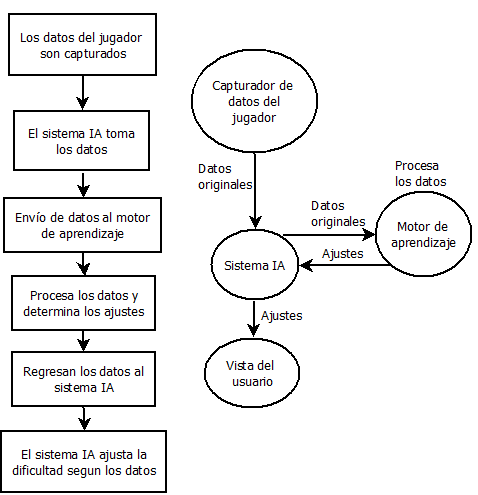
\includegraphics[width=0.5\textwidth]{recursos/Imagenes/Diagrama2Dificultad.png} 
    \caption{Diagrama de vistas del ajuste dinámico de la dificultad}
    \label{fig:mi_imagen}
\end{figure}
\subsection{Sistema de feedback visual y sonoro}
\subsubsection{Diagrama de Vistas del sistema de feedback visual y sonoro}

\begin{figure}[H]
    \centering
    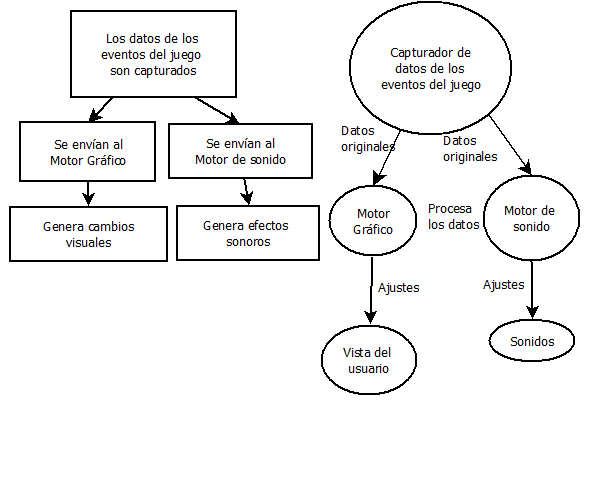
\includegraphics[width=0.5\textwidth]{recursos/Imagenes/Diagrama2Feedback.png} 
    \caption{Diagrama de vistas del sistema de feedback visual y sonoro}
    \label{fig:mi_imagen}
\end{figure}
\subsection{Manejo de guardado de datos}
\subsubsection{Diagrama de Vistas del Manejo de guardado de datos}

\begin{figure}[H]
    \centering
    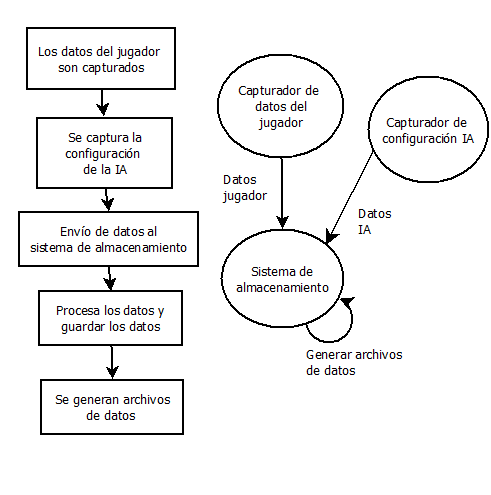
\includegraphics[width=0.5\textwidth]{recursos/Imagenes/Diagrama2GuardaDatos.png} 
    \caption{Diagrama de vistas del manejo de guardado de datos}
    \label{fig:mi_imagen}
\end{figure}


%Diseño del Sistema
\section{Diseño del Sistema}
\subsection{Diagrama de Arquitectura.}

\begin{figure}[htbp]
    \centering
    \adjustbox{width=\textwidth}{
        \begin{tikzpicture}[font=\sffamily,every label/.append
        style={font=\small\sffamily,align=center}]
        \node[cylinder, cylinder uses custom fill, cylinder end fill=blue!25,
        cylinder body fill=blue!50,shape border rotate=90,text=white,
        aspect=0.4,minimum width=1cm,minimum height=1.4cm](Store){BD};
        \node[right=1cm of Store,regular polygon,regular polygon sides=6,fill=orange,
        xscale=1.2,text=white] (Router) {Model IA};
        \node[fit=(Store) (Router)](fit1){};
        \node[below=1cm of fit1,tape, draw,thin, tape bend top=none,fill=purple,
        text=white,minimum width=2.2cm,double copy shadow,minimum height=1.5cm]
        (Components) {Componentes};
        \node[draw,dashed,rounded corners,fit=(Store) (Router) (Components),inner
        sep=10pt,label={above:{Universal\\ Application Code}}](fit2){};
        \node[right=1cm of fit2,doc] (js) {código};
        \node[above right=1cm of js,doc] (Server) {Entidad del\\dispositivo};
        \node[below right=1cm of js,doc] (Client) {Entidad del\\Usuario};
        \draw(fit2.east) -- (js);
        \draw[-latex] (js) |- (Server);
        \draw[-latex] (js) |- (Client);
        \draw[-] (Client) -- ++ (1,0) |- (Server) coordinate[pos=0.25] (aux1);
        \node[draw,dashed,rounded corners,fit=(fit2) (aux1),inner
        xsep=10pt,inner ysep=30pt,label={above:{Source}}](fit3){};
        %
        \pic[right=2cm of aux1,local bounding box=Webpack,scale=2] (Webpack) {pack};
        \node[below=1mm of Webpack,font=\small\sffamily,align=center]{Applicación\\funcional};
        %
        \node[above right=1cm and 2cm of Webpack.east,doc,fill=red!10] (ServerBundle)
        {Paquete de\\Modelos IA};
        \node[below right=1cm and 2cm of Webpack.east,doc,fill=red!10] (ClientBundle) {Paquete de\\Usuarios};
        \node[right=2cm of ServerBundle,parallelepiped,draw=yellow,fill=red!80,
          minimum width=2cm,minimum height=1.5cm,align=center,text=white]
          (BundleRenderer)   {Paquete de\\Paetidas};
        \node[right=2cm of ClientBundle,doc,fill=yellow,minimum width=2cm,minimum height=1.5cm] (HTML) {Estadisticas};
        \draw[-latex] (aux1) -- (Webpack);
        \draw[-latex] (Webpack) -- ++ (2,0) coordinate(aux2) |- (ServerBundle);
        \draw[-latex] (aux2) |- (ClientBundle);
        \draw[-latex] (ClientBundle) -- (HTML) node[midway,below,font=\small\sffamily]{Hydrate};
        \draw (ServerBundle) -- (BundleRenderer);
        \draw[-latex] (BundleRenderer) -- (HTML) node[midway,right,font=\small\sffamily]{Render};
        % 
        \node[draw,dashed,rounded corners,fit=(ServerBundle) (BundleRenderer),inner
        sep=10pt,label={above:{Model server}}](fit4){};
        \node[draw,dashed,rounded corners,fit=(ClientBundle) (HTML),inner
        sep=10pt,label={below:{Statistics Extraction}}](fit5){};
        \end{tikzpicture}
    }
    \caption{Diagrama de la arquitectura de la aplicación.}
    \label{fig:architecture}
\end{figure}
\subsection{Diagrama de Repositorios/BD}
\subsubsection{Diagrama de Flujo de Información}

\usetikzlibrary{positioning, arrows.meta, shapes.geometric, fit, backgrounds}
%\subsubsection{Diagrama de Flujo de Información}
\begin{figure}[H]
\centering
\begin{tikzpicture}[
    entity/.style={rectangle, draw, rounded corners, fill=blue!20, minimum width=2.5cm, minimum height=0.8cm, text centered, font=\small},
    process/.style={rectangle, draw, rounded corners, fill=orange!20, minimum width=3.5cm, minimum height=0.8cm, text centered, font=\small},
    data/.style={cylinder, shape border rotate=90, draw, fill=green!20, minimum width=2cm, minimum height=0.8cm, text centered, font=\small},
    arrow/.style={-{Stealth[scale=1]}, thick},
    every node/.style={font=\small},
    layer/.style={rectangle, draw=none, fill=none}
    ]

    % Definición de Capas
    \matrix[layer, column sep=2cm, row sep=1.5cm]{
        % Primera Columna: Entidades
        \node[entity] (Jugador) {Jugador}; &
        % Segunda Columna: Procesos
        \node[process] (Interfaz) {Interfaz de Usuario y Usabilidad}; &
        \node[process] (Feedback) {Sistema de Feedback Visual y Sonoro}; \\
        \node[entity] (Partida) {Partida}; &
        \node[process] (Generacion) {Generación Procedural de Niveles}; &
        \node[process] (GestionEnemigos) {Gestión de Enemigos y Patrones de Ataque}; \\
        \node[entity] (Nivel) {Nivel}; &
        \node[process] (Registro) {Registro y Análisis de Puntuación}; &
        \node[process] (EntrenamientoIA) {Entrenamiento del Algoritmo de IA}; \\
        \node[entity] (Enemigo) {Enemigo}; &
        \node[process] (IA_Modelo) {IA\_Modelo}; &
        \node[data] (Almacen) {Almacenamiento de Datos}; \\
        \node[entity] (Ataque) {Ataque}; &
        \node[entity] (Estadisticas) {Estadísticas}; &
        \\
    };

    % Conexiones entre Entidades y Procesos
    \draw[arrow] (Jugador) -- (Interfaz) node[midway, above right]{Interactúa};
    \draw[arrow] (Interfaz) -- (Feedback) node[midway, above right]{Envía Eventos};
    \draw[arrow] (Jugador) -- (Partida) node[midway, left]{Juega};
    \draw[arrow] (Partida) -- (Nivel) node[midway, left]{Posee};
    \draw[arrow] (Nivel) -- (Generacion) node[midway, above=.5cm]{Genera Niveles};
    \draw[arrow] (Generacion) -- (Nivel) node[midway, below=.5cm]{Nivel Procedural};
    \draw[arrow] (Partida) -- (Registro) node[midway, left]{Registra Datos};
    \draw[arrow] (Registro) -- (Estadisticas) node[midway, below]{Actualiza};
    \draw[arrow] (Estadisticas) -- (EntrenamientoIA) node[right, below=1cm]{Proporciona Datos};
    \draw[arrow] (EntrenamientoIA) -- (IA_Modelo) node[right, above right=0.5cm]{Actualiza Modelo};
    \draw[arrow] (IA_Modelo) -- (GestionEnemigos) node[right, below right=.5cm]{Modifica};
    \draw[arrow] (GestionEnemigos) -- (Enemigo) node[left,above right=1cm ]{Gestiona};
    \draw[arrow] (Jugador) -- (Ataque) node[midway, above right]{Dispara};
    \draw[arrow] (Enemigo) -- (Ataque) node[midway, above right]{Utiliza};
    \draw[arrow] (Ataque) -- (Feedback) node[right, below right=.5cm]{Feedback de Ataque};
    \draw[arrow] (IA_Modelo) -- (Estadisticas) node[midway, above right]{Genera};
    \draw[arrow] (Almacen) -- (Registro) node[midway, above]{Guarda/Recupera};
    \draw[arrow] (Registro) -- (Almacen) node[midway=2cm, below right=2cm]{Guarda Datos};

    % Ajustes adicionales para evitar solapamientos

\end{tikzpicture}
\caption{Diagrama de Flujo de Información del Proyecto}
\end{figure}

\subsection{Diagrama de interfaces/Interfaces tentativas}
\subsection{Diagrama de interfaces}

\begin{figure}[H]
    \centering
   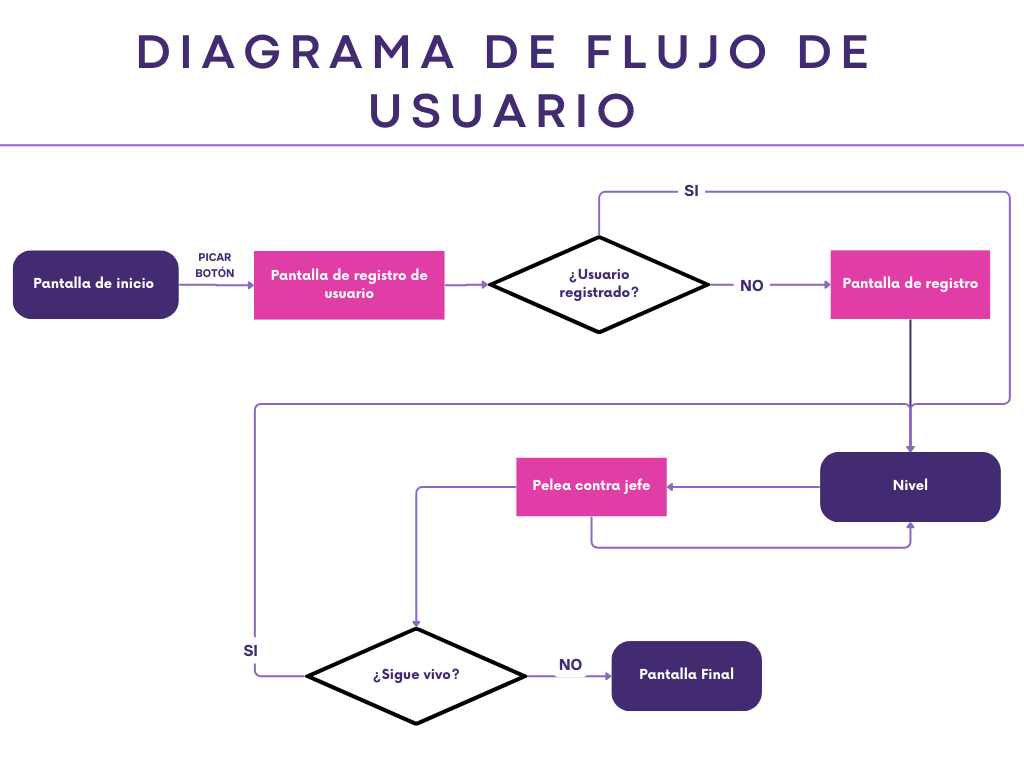
\includegraphics[width=0.5\textwidth]{recursos/Imagenes/Diagrama de Flujo de usuario (1).png} 
    \caption{Diagrama de flujo de usuario}
    \label{fig:mi_imagen}
\end{figure}

\subsection{Posibles interfaces.}
\begin{figure}[H]
    \centering
   
\includegraphics[width=0.5\textwidth]{recursos/Imagenes/Inicio.png} 
    \caption{Primera pantalla}
    \label{fig:mi_imagen}
\end{figure}
\begin{figure}[H]
    \centering
   
\includegraphics[width=0.5\textwidth]{recursos/Imagenes/Ingreso.png} 
    \caption{Ingreso de usuario}
    \label{fig:mi_imagen}
\end{figure}
\begin{figure}[H]
    \centering
   
\includegraphics[width=0.5\textwidth]{recursos/Imagenes/Registro.png} 
    \caption{Registro de usuario}
    \label{fig:mi_imagen}
\end{figure}
\begin{figure}[H]
    \centering
   
\includegraphics[width=0.5\textwidth]{recursos/Imagenes/Nivel.png} 
    \caption{Posible fonde de nivel}
    \label{fig:mi_imagen}
\end{figure}
\begin{figure}[H]
    \centering
   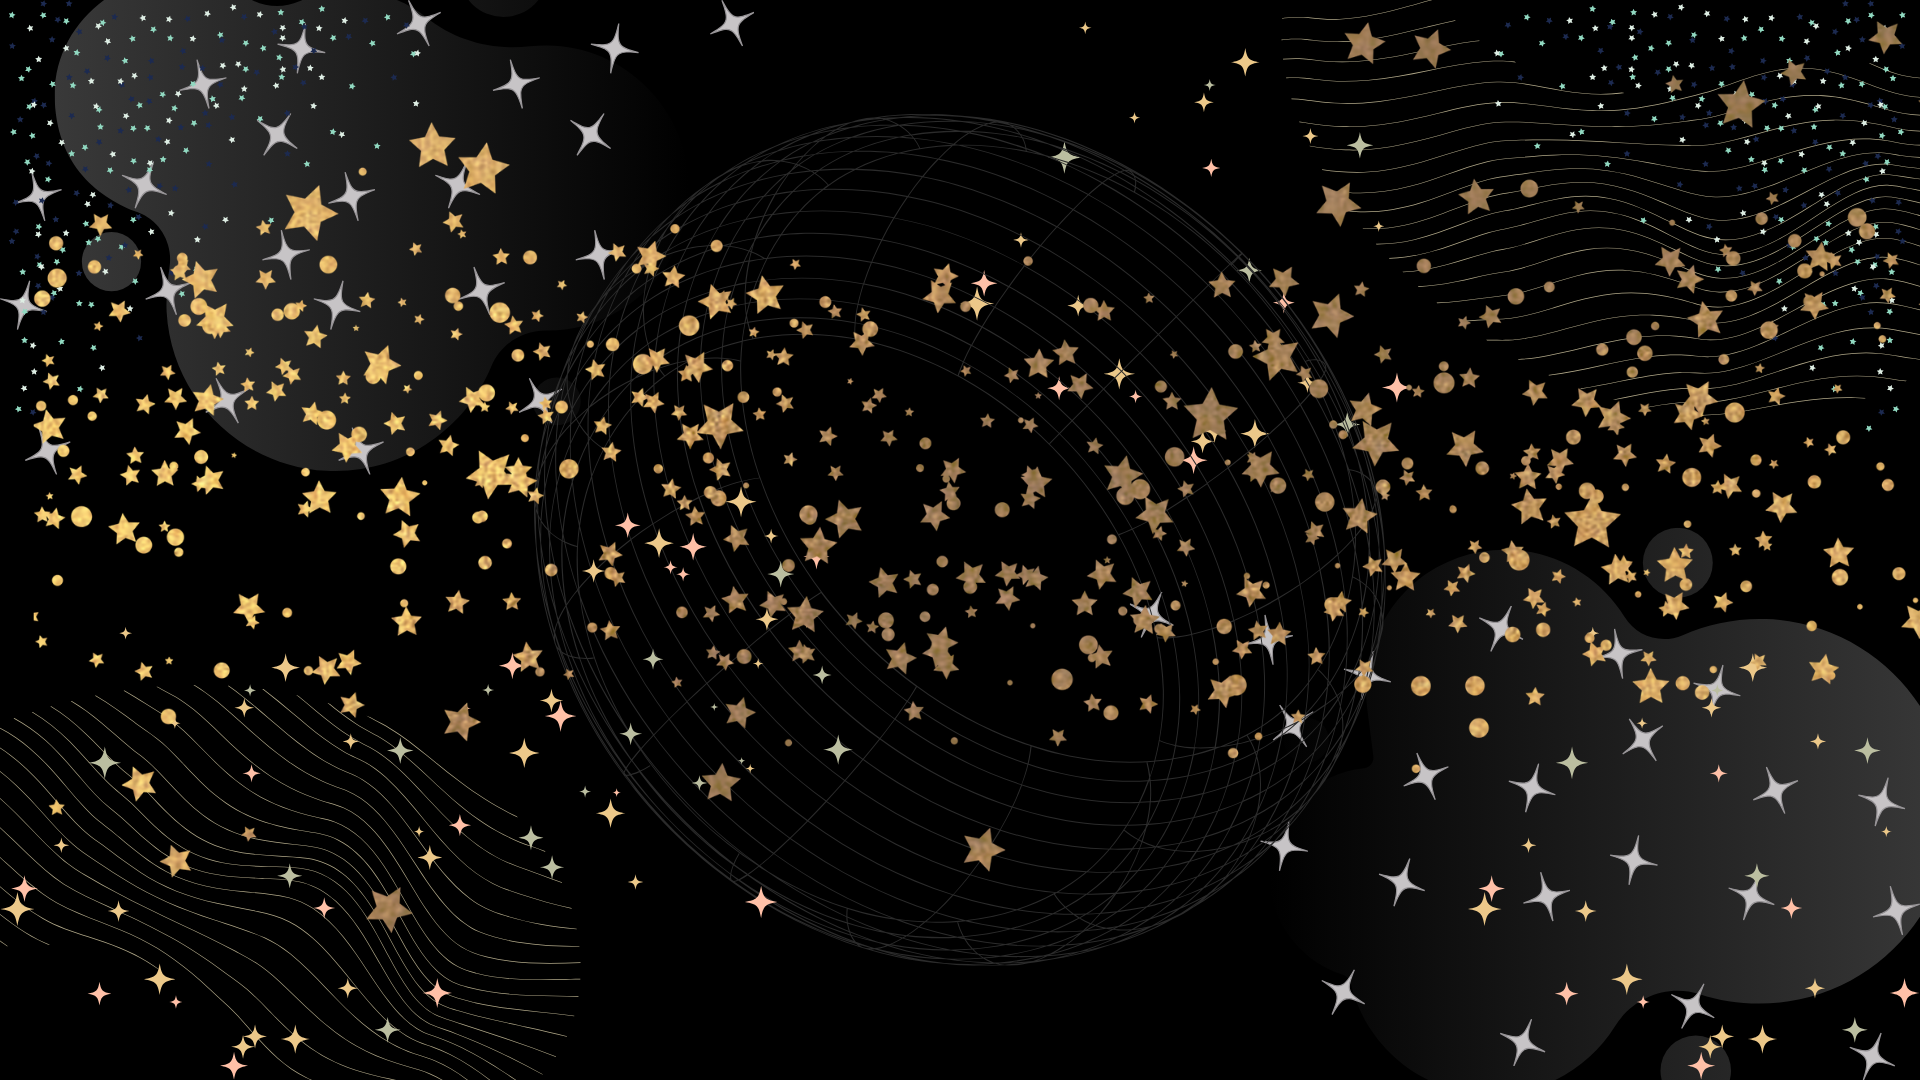
\includegraphics[width=0.5\textwidth]{recursos/Imagenes/Jefe.png} 
    \caption{posible fondo de jefe}
    \label{fig:mi_imagen}
\end{figure}
\begin{figure}[H]
    \centering
   
\includegraphics[width=0.5\textwidth]{recursos/Imagenes/Final partida.png} 
    \caption{Final de partida}
    \label{fig:mi_imagen}
\end{figure}

\subsection{Pseudocodigos.}
\subsubsection{Algoritmos del proceso de \textit{Generación procedural de niveles}.}


\subsubsection*{Algoritmo de Generación Procedural de Entornos}

\textbf{Problemática}: Crear entornos variados pero coherentes. Mantener un equilibrio entre la variedad y la jugabilidad puede ser un reto, ya que demasiada aleatoriedad puede generar niveles desequilibrados o imposibles de completar.

\textbf{Posible solución}: Utilización de algoritmos como \textit{Perlin Noise} o \textit{Simplex Noise} para generar terrenos o plataformas con una coherencia visual y de estructura. También se pueden emplear \textit{gramáticas de espacio} para la disposición de ambientes más estructurados.

\textbf{Desafío técnico}: Mantener un balance entre la generación aleatoria y las reglas del diseño de niveles. Es necesario verificar que los niveles generados sean accesibles y jugables (sin zonas inalcanzables).

\begin{algorithm}
\caption{Inicializar Generador de Terrenos (e.g., Perlin Noise)\;}
\SetAlgoLined
\ForEach{sector del nivel}{
    Definir parámetros de terreno (altura, bioma, etc.)\;
    Generar altura usando ruido (Perlin Noise)\;
    \If{bioma == 'agua'}{
        Establecer zona como agua\;
    }
    \ElseIf{bioma == 'montaña'}{
        Establecer elevación adicional\;
    }
}
Verificar que no haya zonas inalcanzables\;
\ForEach{punto de inicio y final}{
    \If{distancia(punto inicio, punto final) no es accesible}{
        Ajustar terreno o generar puente/plataforma\;
    }
}
\Return{entorno generado}
\end{algorithm}

\subsubsection*{Algoritmo de Distribución de Obstáculos}

\textbf{Problemática}: La colocación de obstáculos debe respetar reglas de accesibilidad, sin hacer el nivel demasiado difícil ni demasiado fácil.

\textbf{Posible solución}: Algoritmos de \textit{optimización espacial} como \textit{temple simulado (simulated annealing)} o algoritmos genéticos pueden ser útiles para iterar sobre las colocaciones de obstáculos y ajustar la dificultad, evitando repeticiones no deseadas y respetando restricciones de espacio.

\textbf{Desafío técnico}: La necesidad de verificar constantemente que la disposición de los obstáculos no bloquee el progreso del jugador y que ofrezca un reto adecuado.

\begin{algorithm}
\SetAlgoLined
\caption{Inicializar Lista de Obstáculos (paredes, trampas, bloques)};
Definir la cantidad máxima de obstáculos según la dificultad\;
\ForEach{sector del nivel}{
    Seleccionar una ubicación aleatoria\;
    Verificar que la ubicación sea accesible\;
    Colocar obstáculo\;
    Evaluar balance de dificultad\;
    \If{dificultad > límite superior}{
        Eliminar obstáculos o reubicar\;
    }
}
Iterar hasta lograr una distribución óptima usando algoritmo de temple simulado\;
Ajustar distribución según las restricciones (accesibilidad, dificultad)\;
\Return{obstáculos distribuidos}
\end{algorithm}

\subsubsection*{Algoritmo de Distribución de Enemigos}

\textbf{Problemática}: Colocar enemigos de manera estratégica en el nivel, ajustando su comportamiento según la dificultad del jugador, puede volverse complicado en niveles más avanzados o con enemigos complejos.

\textbf{Posible solución}: Usar una \textit{red neuronal o aprendizaje profundo} para ajustar dinámicamente la colocación y el comportamiento de los enemigos basándose en el estilo de juego del usuario (un enfoque de dificultad adaptativa). Alternativamente, un enfoque de \textit{clusterización jerárquica} podría agrupar enemigos según el espacio disponible o su dificultad para asegurarse de que no se concentren en un solo punto.

\textbf{Desafío técnico}: El cálculo eficiente y adaptativo del comportamiento enemigo en tiempo real, asegurando que los enemigos estén bien distribuidos pero sin predecir el comportamiento del jugador con demasiada precisión, lo que podría hacer el juego frustrante o repetitivo.

\begin{algorithm}
\caption{Inicializar Lista de Enemigos disponibles};
\SetAlgoLined
Definir cantidad y tipo de enemigos según la dificultad del jugador\;
\ForEach{sector del nivel}{
    Seleccionar una posición estratégica aleatoria\;
    Colocar enemigo en la posición\;
}
Ajustar el comportamiento enemigo según la dificultad del jugador\;
\If{jugador es avanzado}{
    Aumentar agresividad y velocidad\;
}
\ElseIf{jugador es novato}{
    Reducir agresividad y añadir enemigos más fáciles\;
}
Verificar que los enemigos estén bien distribuidos\;
\If{enemigos están demasiado cerca o concentrados}{
    Reubicar algunos de ellos\;
}
\Return{nivel con enemigos colocados};
\end{algorithm}
\subsubsection*{Algoritmo de Ajuste Dinámico de Dificultad}

\textbf{Problemática}: Ajustar la dificultad en función del rendimiento del jugador sin hacer el juego ni demasiado fácil ni demasiado difícil.

\textbf{Posible solución}: Se puede usar un sistema de \textit{aprendizaje reforzado} que ajuste los parámetros del juego (como la cantidad de enemigos, su agresividad o la cantidad de obstáculos) en función del comportamiento del jugador. Este sistema podría aprender del jugador en tiempo real y ajustar las condiciones del nivel en consecuencia.

\textbf{Desafío técnico}: El ajuste de dificultad debe realizarse de manera sutil para que el jugador no perciba cambios drásticos, lo que podría afectar la inmersión. También es crucial evitar la creación de “picos” de dificultad que hagan el juego injustamente complicado.

\begin{algorithm}
\caption{Inicializar parámetros de dificultad (agresividad, cantidad de enemigos, velocidad, etc.).}
\SetAlgoLined
Monitorear el desempeño del jugador (e.g., precisión, tiempo de reacción)\;
\ForEach{nivel generado}{
    Ajustar dificultad dinámicamente\;
    \If{jugador progresa muy rápido}{
        Incrementar cantidad de enemigos o agresividad\;
    }
    \ElseIf{jugador tiene dificultades}{
        Reducir la cantidad de enemigos o facilitar obstáculos\;
    }
}
Aplicar los ajustes al nivel en tiempo real\;
\Return{nivel ajustado con la dificultad adaptada}\;
\end{algorithm}

\subsubsection*{Algoritmo de Verificación de Reglas}

\textbf{Problemática}: Asegurar que el nivel generado sea jugable y cumpla con las reglas establecidas (accesibilidad, distribución de enemigos y obstáculos, etc.).

\textbf{Posible solución}: Un \textit{algoritmo de búsqueda} como \textit{A* (A-star)} o \textit{algoritmos basados en grafos} para verificar que cada parte del nivel sea accesible y jugable. El algoritmo puede validar la disposición de los obstáculos y enemigos y confirmar que el jugador puede completar el nivel sin quedar atrapado o encontrarse en situaciones imposibles.

\textbf{Desafío técnico}: Verificar las reglas sin impactar negativamente en el rendimiento del juego, especialmente en niveles muy complejos o con una gran cantidad de elementos.

\begin{algorithm}
\caption{Algoritmo de verificación de Reglas}
\SetAlgoLined
\ForEach{sector del nivel generado}{
    Generar un grafo representando el mapa\;
    Ejecutar el algoritmo A* para verificar rutas accesibles\;
    \If{ruta no es accesible}{
        Ajustar el terreno o reubicar obstáculos\;
    }
    Verificar la distribución de enemigos y obstáculos\;
    \If{enemigos u obstáculos bloquean el progreso}{
        Reubicar elementos\;
    }
}
\If{el nivel cumple con las reglas de jugabilidad}{
    \Return{``Verificación exitosa''}\;
}
\Else{
    \Return{``Ajustes necesarios''}\;
}
\end{algorithm}

\subsubsection*{Algoritmo de Generación de Entornos Jugables}

\textbf{Problemática}: Asegurarse de que los niveles generados sean divertidos, equilibrados y no repetitivos, mientras se ajustan a las reglas de diseño establecidas.

\textbf{Posible solución}: \textit{Algoritmos basados en evolución procedural} (PCG - Procedural Content Generation) que usan \textit{gramáticas generativas} o métodos como \textit{Markov Chains} para crear niveles con ciertas estructuras reconocibles, pero que aún mantienen variedad.

\textbf{Desafío técnico}: Evitar la monotonía, asegurando que el sistema pueda generar suficientes variaciones interesantes en los niveles para que el jugador no perciba repetición en la experiencia.

\begin{algorithm}
\caption{Generación Procedural de un Nivel Jugable}
\SetAlgoLined

Inicializar gramática procedural para generar estructuras reconocibles\;
\ForEach{sector del nivel}{
    Generar secciones del nivel utilizando gramáticas\;
    Validar la jugabilidad de cada sección (rutas, obstáculos, enemigos)\;
}
Evaluar el balance de dificultad y variedad\;
\If{sección es muy repetitiva}{
    Cambiar parámetros para generar una variación\;
}
Verificar accesibilidad\;
\If{alguna sección no es accesible}{
    Ajustar su generación\;
}
\Return{Entorno jugable generado}\;
\end{algorithm}
\subsubsection{Algoritmos del proceso de \textit{Ajuste Dinamico de Dificultad.}}
\subsubsection*{Algoritmo de Ajuste Dinámico de Dificultad}

\textbf{Problemática}: Ajustar la dificultad en función del rendimiento del jugador sin hacer el juego ni demasiado fácil ni demasiado difícil.

\textbf{Posible solución}: Se puede usar un sistema de \textit{aprendizaje reforzado} que ajuste los parámetros del juego (como la cantidad de enemigos, su agresividad o la cantidad de obstáculos) en función del comportamiento del jugador. Este sistema podría aprender del jugador en tiempo real y ajustar las condiciones del nivel en consecuencia.

\textbf{Desafío técnico}: El ajuste de dificultad debe realizarse de manera sutil para que el jugador no perciba cambios drásticos, lo que podría afectar la inmersión. También es crucial evitar la creación de “picos” de dificultad que hagan el juego injustamente complicado.


\subsection*{Entradas:}
\begin{itemize}
    \item Datos del jugador:
    \begin{itemize}
        \item vidas\_perdidas
        \item precision
        \item puntuacion
    \end{itemize}
\end{itemize}

\subsection*{Salidas:}
\begin{itemize}
    \item Modificaciones de la dificultad:
    \begin{itemize}
        \item numero\_enemigos
        \item velocidad\_enemigos
        \item patrones\_enemigos
    \end{itemize}
\end{itemize}

\subsection*{Actores:}
\begin{itemize}
    \item Sistema de IA
    \item Motor de aprendizaje
\end{itemize}

\subsection*{Pseudocódigo:}
\begin{algorithm}[H]
\caption{Ajuste Dinámico de la Dificultad del Juego}
\SetAlgoLined
\KwIn{vidas\_perdidas, precision, puntuacion}
\KwOut{numero\_enemigos, velocidad\_enemigos, patrones\_enemigos}

\BlankLine
\tcp{Inicialización de parámetros}
dificultad\_base $\leftarrow$ 1.0\;
incremento\_dificultad $\leftarrow$ 0.1\;
vidas\_max $\leftarrow$ 3\;
precision\_esperada $\leftarrow$ 0.75\;
puntuacion\_esperada $\leftarrow$ 1000\;

\While{el juego esté en ejecución}{
    \tcp{Leer datos del jugador}
    leer(vidas\_perdidas, precision, puntuacion)\;

    \If{vidas\_perdidas > 0}{
        dificultad\_base $\leftarrow$ dificultad\_base - \dfrac{vidas\_perdidas}{vidas\_max}\;
    }

    \If{precision < precision\_esperada}{
        dificultad\_base $\leftarrow$ dificultad\_base - incremento\_dificultad\;
    }

    \If{puntuacion $\geq$ puntuacion\_esperada}{
        dificultad\_base $\leftarrow$ dificultad\_base + incremento\_dificultad\;
    }

    \tcp{Aplicar límites a la dificultad}
    dificultad\_base $\leftarrow$ \texttt{max}(0.5, \texttt{min}(dificultad\_base, 2.0))\;

    \tcp{Modificar parámetros de enemigos según la dificultad}
    numero\_enemigos $\leftarrow$ base\_enemigos * dificultad\_base\;
    velocidad\_enemigos $\leftarrow$ base\_velocidad * dificultad\_base\;
    patrones\_enemigos $\leftarrow$ seleccionar\_patrones(dificultad\_base)\;

    \tcp{Enviar parámetros ajustados al motor de juego}
    enviar\_parametros(numero\_enemigos, velocidad\_enemigos, patrones\_enemigos)\;

    \tcp{Actualizar datos del jugador con retroalimentación del sistema IA y motor de aprendizaje}
    actualizar\_datos\_jugador()\;
}

\end{algorithm}

\subsection*{Explicación:}
El sistema ajusta dinámicamente la dificultad del juego basándose en el rendimiento del jugador. Si el jugador pierde vidas o su precisión cae por debajo del umbral esperado, la dificultad se reduce. Si la puntuación supera la esperada, la dificultad aumenta. El ajuste se aplica a los enemigos, modificando su número, velocidad y patrones. El motor de aprendizaje recibe retroalimentación para mejorar la adaptación del sistema a largo plazo.

\subsubsection{Algoritmos del proceso del \textit{modelo de IA}}
\subsubsection*{Algoritmo de Validación de Datos Históricos (Vista Lógica y Física)}
\textbf{Problemática}: Verificar que los datos de las partidas sean válidos y consistentes antes de usarlos en el modelo de IA.

\begin{algorithm}[H]
\caption{Validación de Datos Históricos}
\SetAlgoLined
\KwIn{Datos\_Históricos}
\ForEach{partida en Datos\_Históricos}{
    \If{partida.puntuacion < 0 \textbf{or} partida.precision < 0 \textbf{or} partida.tiempo\_jugado <= 0}{
        Descartar partida\;
    }
    \If{partida.vidas\_perdidas < 0 \textbf{or} partida.enemigos\_eliminados < 0}{
        Descartar partida\;
    }
    \If{datos inconsistentes encontrados}{
        Notificar error y corregir\;
    }
}
\Return{Datos\_Históricos\_Validados}
\end{algorithm}

\subsubsection*{Algoritmo de Preprocesamiento de Datos.}
\textbf{Problemática}: Preparar los datos recopilados para ser utilizados en el entrenamiento del modelo de IA, mediante normalización y generación de nuevas características.

\begin{algorithm}[H]
\caption{Preprocesamiento de Datos}
\SetAlgoLined
\KwIn{Datos\_Históricos\_Validados}
Datos\_Normalizados = Normalizar(Datos\_Históricos\_Validados)\;
Caracteristicas\_Adicionales = Generar\_Caracteristicas(Datos\_Normalizados)\;
\ForEach{partida en Caracteristicas\_Adicionales}{
    tendencia = Calcular\_Tendencia(partida.puntuacion, partida.precision, partida.vidas\_perdidas)\;
    Agregar tendencia a partida\;
}
\Return{Datos\_Preprocesados}
\end{algorithm}

\begin{algorithm}[H]
\caption{Normalización de Datos}
\SetAlgoLined
\KwIn{Datos}
\ForEach{dato en Datos}{
    dato.normalizado = $\frac{dato.valor - min(dato)}{max(dato) - min(dato)}$\;
}
\Return{Datos\_Normalizados}
\end{algorithm}

\begin{algorithm}[H]
\caption{Generación de Características}
\SetAlgoLined
\KwIn{Datos}
Crear nuevas características basadas en estadísticas (p. ej., mejora del rendimiento del jugador en cada partida)\;
\Return{Datos con características adicionales}
\end{algorithm}

\subsubsection*{Algoritmo de Entrenamiento del Modelo.}
\textbf{Problemática}: Entrenar un modelo de red neuronal basado en los datos preprocesados, ajustando los pesos mediante retropropagación.

\begin{algorithm}[H]
\caption{Entrenamiento del Modelo}
\SetAlgoLined
\KwIn{Datos\_Preprocesados}
Inicializar modelo con pesos aleatorios\;
\ForEach{época}{
    \ForEach{entrada en Datos\_Preprocesados}{
        salida\_predicha = Propagar\_Adelante(entrada, modelo)\;
        error = Calcular\_Error(salida\_predicha, entrada.objetivo)\;
        Ajustar\_Pesos(error, modelo)\;
        Retropropagar(error, modelo)\;
    }
}
\Return{Modelo\_Entrenado}
\end{algorithm}

\begin{algorithm}[H]
\caption{Propagación Adelante}
\SetAlgoLined
\KwIn{entrada, modelo}
\ForEach{capa en modelo}{
    entrada = Activacion(Suma\_Pesos(entrada, capa.pesos))\;
}
\Return{entrada como salida\_predicha}
\end{algorithm}

\begin{algorithm}[H]
\caption{Ajuste de Pesos}
\SetAlgoLined
\KwIn{error, modelo}
\ForEach{capa en modelo}{
    Actualizar pesos basándose en error y tasa de aprendizaje\;
}
\end{algorithm}

\begin{algorithm}[H]
\caption{Retropropagación}
\SetAlgoLined
\KwIn{error, modelo}
Propagar el error hacia atrás ajustando pesos de capas anteriores\;
\end{algorithm}

\subsubsection*{Algoritmo de Evaluación del Modelo.}
\textbf{Problemática}: Evaluar el rendimiento del modelo entrenado utilizando métricas clave.

\begin{algorithm}[H]
\caption{Evaluación del Modelo}
\SetAlgoLined
\KwIn{Modelo\_Entrenado, Datos\_Validacion}
métrica\_precision = 0\;
métrica\_tiempo\_respuesta = 0\;
\ForEach{entrada en Datos\_Validacion}{
    predicción = Modelo\_Entrenado.Propagar\_Adelante(entrada)\;
    métrica\_precision += Comparar\_Prediccion(predicción, entrada.objetivo)\;
    métrica\_tiempo\_respuesta += Calcular\_Tiempo\_Respuesta(predicción)\;
}
Calcular\_Métricas\_Finales(métrica\_precision, métrica\_tiempo\_respuesta)\;
\Return{Métricas}
\end{algorithm}

\begin{algorithm}[H]
\caption{Comparación de Predicción}
\SetAlgoLined
\KwIn{predicción, objetivo}
\If{predicción es correcta}{
    \Return{1}\;
}
\Else{
    \Return{0}\;
}
\end{algorithm}

\begin{algorithm}[H]
\caption{Cálculo del Tiempo de Respuesta}
\SetAlgoLined
\KwIn{predicción}
Medir tiempo que tomó la predicción\;
\Return{tiempo}
\end{algorithm}

\subsubsection*{Algoritmo de Ajuste de Parámetros.}
\textbf{Problemática}: Ajustar los parámetros del modelo si el rendimiento es subóptimo según las métricas evaluadas.

\begin{algorithm}[H]
\caption{Ajuste de Parámetros del Modelo}
\SetAlgoLined
\KwIn{Modelo\_Entrenado, Métricas}
\If{Métricas.precision < umbral \textbf{or} Métricas.tiempo\_respuesta > limite}{
    Ajustar tasa\_de\_aprendizaje en Modelo\_Entrenado\;
    Aumentar número de iteraciones si es necesario\;
    Reentrenar el modelo con los nuevos parámetros\;
}
\Return{Modelo\_Ajustado}
\end{algorithm}

\subsubsection*{Algoritmo de Implementación del Modelo Actualizado.}
\textbf{Problemática}: Integrar el modelo actualizado en el sistema de juego para ajustar la dificultad en tiempo real.

\begin{algorithm}[H]
\caption{Implementación del Modelo}
\SetAlgoLined
\KwIn{Modelo\_Ajustado}
Sistema\_Juego.Cargar\_Modelo(Modelo\_Ajustado)\;
\While{juego esté activo}{
    Datos\_Actuales = Recopilar\_Datos\_Juego()\;
    dificultad\_ajustada = Modelo\_Ajustado.Prediccion(Datos\_Actuales)\;
    Sistema\_Juego.Ajustar\_Dificultad(dificultad\_ajustada)\;
}
\end{algorithm}

\subsubsection{Algoritmos del proceso de \textit{Retroalimentacion Visual y Sonora en Tiempo Real.}}

\subsection*{Problemática}
En muchos juegos, proporcionar retroalimentación inmediata al jugador es crucial para mejorar la inmersión y la experiencia de juego. Sin embargo, gestionar esta retroalimentación visual y sonora en tiempo real puede ser un desafío, especialmente cuando se debe reaccionar dinámicamente a varios eventos de juego, tales como:
\begin{itemize}
    \item Derrotas.
    \item Cambios en la dificultad.
    \item Logros alcanzados.
    \item Avances en niveles.
\end{itemize}

Los principales problemas son:
\begin{itemize}
    \item Desincronización entre los eventos del juego y la retroalimentación visual o sonora.
    \item Falta de personalización de la retroalimentación basada en la complejidad de los eventos.
    \item Sobrecarga de recursos si la retroalimentación no se gestiona eficientemente, lo que puede provocar retrasos o bloqueos.
\end{itemize}

\subsection*{Posible Solución}
El algoritmo de retroalimentación visual y sonora en tiempo real tiene como objetivo sincronizar los eventos del juego con respuestas visuales (sprites) y sonoras (efectos) adecuadas. La solución consiste en:
\begin{itemize}
    \item \textbf{Detectar eventos clave en el juego:} Lectura de eventos durante la ejecución, como derrotas, cambios en la dificultad, logros y avances.
    \item \textbf{Proporcionar retroalimentación visual:} Mostrar sprites en ubicaciones apropiadas, como explosiones al perder o íconos cuando aumenta la dificultad.
    \item \textbf{Proporcionar retroalimentación sonora:} Reproducir sonidos que refuercen la experiencia del jugador, como sonidos para logros o cambios de dificultad.
    \item \textbf{Sincronización con el motor de juego:} Asegurar que los sprites y efectos sonoros se envíen al motor gráfico y de sonido sin latencia perceptible.
\end{itemize}

\subsection*{Desafío Técnico}
Implementar esta solución de retroalimentación visual y sonora en tiempo real presenta varios desafíos técnicos, incluyendo:

\textbf{Sincronización en tiempo real}
El sistema debe reaccionar de forma instantánea a los eventos. Cualquier retraso en la detección de los eventos o en la representación visual/sonora afectaría negativamente la experiencia del jugador. El algoritmo debe ser lo suficientemente eficiente para evitar un lag perceptible.

\textbf{Gestión de múltiples eventos simultáneos}
El sistema debe ser capaz de manejar varios eventos ocurriendo al mismo tiempo. Por ejemplo, si un jugador pierde una vida mientras logra un objetivo, el sistema debe mostrar tanto la derrota como el logro sin sobrecargar el motor gráfico o de sonido.

\textbf{Optimización de recursos}
Para evitar la sobrecarga del sistema, es necesario gestionar cuidadosamente las llamadas al motor gráfico y de sonido. Esto incluye evitar redundancias en los efectos de sonido y la superposición innecesaria de sprites.

\textbf{Escalabilidad}
A medida que el juego se vuelve más complejo, con más eventos posibles, el sistema debe poder escalar sin comprometer el rendimiento. El motor de retroalimentación debe ser capaz de manejar desde juegos simples hasta títulos más complejos sin perder fluidez.


\subsection*{Entradas:}
\begin{itemize}
    \item Eventos del juego:
    \begin{itemize}
        \item derrotas
        \item cambios\_dificultad
        \item logros
        \item avances
    \end{itemize}
\end{itemize}

\subsection*{Salidas:}
\begin{itemize}
    \item Indicaciones visuales y sonoras:
    \begin{itemize}
        \item sprites
        \item efectos\_sonido
    \end{itemize}
\end{itemize}

\subsection*{Actores:}
\begin{itemize}
    \item Motor gráfico
    \item Motor de sonido
\end{itemize}

\subsection*{Pseudocódigo:}
\begin{algorithm}[H]
\caption{Retroalimentación Visual y Sonora en Tiempo Real}
\SetAlgoLined
\KwIn{derrotas, cambios\_dificultad, logros, avances}
\KwOut{sprites, efectos\_sonoros}

\While{el juego esté en ejecución}{
    \tcp{Leer eventos del juego}
    leer(eventos)\;

    \If{evento == derrota}{
        \tcp{Retroalimentación para derrotas}
        mostrar\_sprite("explosion", posicion\_jugador)\;
        reproducir\_sonido("derrota")\;
    }

    \If{evento == cambios\_dificultad}{
        \If{dificultad aumenta}{
            \tcp{Retroalimentación para aumento de dificultad}
            mostrar\_sprite("icono\_dificultad\_up", pantalla)\;
            reproducir\_sonido("dificultad\_aumenta")\;
        }
        \If{dificultad disminuye}{
            \tcp{Retroalimentación para disminución de dificultad}
            mostrar\_sprite("icono\_dificultad\_down", pantalla)\;
            reproducir\_sonido("dificultad\_disminuye")\;
        }
    }

    \If{evento == logro}{
        \tcp{Retroalimentación para logros}
        mostrar\_sprite("icono\_logro", centro\_pantalla)\;
        reproducir\_sonido("logro\_desbloqueado")\;
    }

    \If{evento == avance}{
        \tcp{Retroalimentación para avances en el juego}
        mostrar\_sprite("indicador\_avance", interfaz)\;
        reproducir\_sonido("avanzar\_nivel")\;
    }

    \tcp{Enviar sprites y efectos sonoros al motor gráfico y de sonido}
    enviar\_sprites\_y\_sonidos(motor\_grafico, motor\_sonido)\;
}

\end{algorithm}

\subsection*{Explicación:}
Este pseudocódigo gestiona los eventos del juego como derrotas, cambios en la dificultad, logros y avances. Dependiendo del evento, se generan indicaciones visuales (sprites) y sonoras (efectos de sonido) que son enviadas al motor gráfico y al motor de sonido. Por ejemplo, al perder una vida, se muestra un sprite de explosión y se reproduce un sonido específico de derrota. De igual manera, si hay un cambio en la dificultad o se alcanza un logro, la retroalimentación visual y sonora se adapta.


\subsubsection{Algoritmos del proceso d\textit{Gestión de enemigos y patrón de ataques}}

\subsubsection*{Algoritmo de Selección de Enemigos y Patrones de Ataque}
\textbf{Problemática}: Seleccionar enemigos adecuados y generar patrones de ataque en tiempo real basados en variables de dificultad.\\
\textbf{Algoritmo}: Se puede usar una \textit{heurística de selección} combinada con un \textit{algoritmo de búsqueda} como \textit{algoritmo genético}. Los enemigos y sus patrones de ataque se seleccionan según la dificultad, iterando sobre un conjunto de posibles combinaciones y eligiendo las más optimizadas según el nivel actual.\\
\textbf{Desafío}: Adaptarse en tiempo real a los cambios en la dificultad y garantizar que los patrones generados no sean repetitivos ni imposibles.

\begin{algorithm}[H]
\caption{Algoritmo Genético para Selección de Enemigos y Patrones de Ataque}
\SetAlgoLined

Inicializar población con N configuraciones de enemigos y patrones\;
\ForEach{configuración en la población}{
    Evaluar cada configuración en base a:
    \begin{itemize}
        \item Dificultad deseada
        \item Diversidad de patrones
        \item Repetición de ataques
    \end{itemize}
}

\For{cada iteración hasta el número máximo de generaciones}{
    Seleccionar configuraciones más óptimas (por ejemplo, mediante torneo)\;
    Cruzar las configuraciones seleccionadas para generar nuevas combinaciones\;
    Mutar aleatoriamente algunos patrones en las nuevas configuraciones\;
    Evaluar nuevas configuraciones\;
    \If{se encuentra una configuración óptima o se alcanzan las generaciones máximas}{
        Salir del bucle\;
    }
}
\Return{configuración más adecuada para la situación actual del juego}\;

\end{algorithm}

\subsubsection*{Algoritmo de Ajuste Dinámico de Ataques}
\textbf{Problemática}: Ajustar el comportamiento de los enemigos y sus patrones de ataque en función del rendimiento del jugador en tiempo real.\\
\textbf{Algoritmo}: El uso de un \textit{sistema basado en aprendizaje reforzado} o un \textit{modelo predictivo} que ajuste patrones de ataque dinámicamente, aprendiendo del estilo de juego del usuario y modificando la dificultad de manera progresiva.\\
\textbf{Desafío}: Mantener una transición suave en los ajustes, evitando cambios bruscos que puedan desbalancear la jugabilidad.

\begin{algorithm}[H]
\caption{Ajuste dinámico de ataques basado en Aprendizaje Reforzado}
\SetAlgoLined

Inicializar un modelo de Aprendizaje Reforzado (Q-learning o similar)\;
Definir estados (niveles de rendimiento del jugador)\;
Definir acciones (ajustes en patrones de ataque: más agresivo, más defensivo, etc.)\;
Definir recompensas (basado en si el jugador mejora o empeora)\;

\While{el juego esté en progreso}{
    Observar el rendimiento del jugador\;
    Determinar el estado actual del jugador\;
    Elegir la mejor acción basada en el modelo actual (exploración vs explotación)\;
    Ejecutar el ajuste de patrones de ataque\;
    Observar el resultado (mejora o empeora la experiencia del jugador)\;
    Actualizar el modelo de aprendizaje reforzado basado en la recompensa obtenida\;
}

Actualizar patrones de ataque dinámicamente según la acción seleccionada\;

\end{algorithm}


\subsubsection*{Algoritmo de Gestión de Variables de Dificultad}
\textbf{Problemática}: Recopilar y procesar datos como estadísticas del jugador y variables de dificultad para generar ataques adecuados.\\
\textbf{Algoritmo}: Un \textit{algoritmo de clasificación jerárquica} podría agrupar los datos del jugador (rendimiento, estadísticas) y decidir cómo influir en los parámetros de ataque. Por ejemplo, clasificar los jugadores en diferentes niveles de habilidad para ajustar la agresividad de los enemigos.\\
\textbf{Desafío}: Procesar los datos en tiempo real sin sobrecargar el sistema o causar retrasos en la jugabilidad.

\begin{algorithm}[H]
\caption{Algoritmo de Clasificación Jerárquica para Variables de Dificultad}
\SetAlgoLined

Inicializar datos de rendimiento del jugador (estadísticas como precisión, tiempo de reacción, etc.)\;
Agrupar jugadores en diferentes niveles de habilidad mediante Clasificación Jerárquica\;

\While{el juego esté en progreso}{
    Recoger datos de rendimiento del jugador en tiempo real\;
    Actualizar la clasificación del jugador si es necesario\;

    \uIf{el jugador pertenece al grupo de nivel bajo}{
        Generar patrones de ataque menos agresivos\;
    }
    \uElseIf{el jugador pertenece al grupo de nivel medio}{
        Generar patrones balanceados\;
    }
    \ElseIf{el jugador pertenece al grupo de nivel alto}{
        Generar patrones más agresivos\;
    }
}

Actualizar constantemente los ataques según la nueva clasificación\;
\end{algorithm}

\subsubsection*{Algoritmo de Control de Carga}
\textbf{Problemática}: Garantizar que el ajuste dinámico y generación de enemigos/patrones de ataque no afecte negativamente el rendimiento del juego.\\
\textbf{Algoritmo}: Se puede implementar un \textit{algoritmo de control de rendimiento} basado en la cantidad de enemigos y la complejidad del patrón de ataque. Técnicas como el \textit{cálculo incremental} o el \textit{ajuste procedural limitado} pueden ayudar a mantener el equilibrio.\\
\textbf{Desafío}: Lograr un rendimiento estable incluso en niveles muy complejos, con múltiples enemigos y patrones de ataque en pantalla.

\begin{algorithm}[H]
\caption{Control de Carga para Manejo de Enemigos y Patrones}
\SetAlgoLined

Definir límite máximo de enemigos y complejidad de patrones basado en los recursos del sistema\;
Inicializar la cantidad de enemigos y la complejidad de patrones a un nivel básico\;

\While{el juego esté en progreso}{
    Medir uso de CPU y GPU del sistema\;

    \uIf{el uso del sistema es bajo}{
        Aumentar la cantidad de enemigos y la complejidad de los patrones\;
    }
    \uElseIf{el uso del sistema está cerca del límite}{
        Reducir la cantidad de enemigos o simplificar los patrones de ataque\;
    }
}

Ajustar dinámicamente la cantidad de enemigos y la complejidad según el rendimiento del sistema\;

\end{algorithm}

\subsubsection*{Algoritmo de Sincronización de Módulos}
\textbf{Problemática}: Integrar la gestión de enemigos con otros sistemas como el motor procedural de niveles o el ajuste de dificultad adaptativa.\\
\textbf{Algoritmo}: Un \textit{algoritmo de sincronización} basado en eventos podría coordinar las funciones de los diferentes módulos. Por ejemplo, cuando el nivel se genera, el sistema de enemigos debe ser notificado para colocar adecuadamente los enemigos.\\
\textbf{Desafío}: Asegurarse de que la comunicación entre los sistemas sea eficiente y sincrónica, sin causar cuellos de botella en el rendimiento.

\begin{algorithm}[H]
\caption{Algoritmo de Sincronización de Módulos basado en eventos}
\SetAlgoLined

\When{el nivel se genera}{
    Notificar al sistema de gestión de enemigos\;
    Obtener la estructura del nivel generado\;
    \ForEach{región del nivel}{
        Asignar enemigos y patrones de ataque adecuados\;
    }
    Sincronizar el sistema de IA con el entorno generado\;
    Notificar al sistema de ajuste dinámico de dificultad\;
}

\When{los parámetros del jugador cambien}{
    Ajustar los patrones de ataque en consecuencia\;
    Actualizar otros módulos según los nuevos parámetros (dificultad, enemigos)\;
}

Coordinar la comunicación entre módulos para asegurar consistencia\;

\end{algorithm}


\subsubsection*{Algoritmo de Verificación de Jugabilidad}
\textbf{Problemática}: Asegurar que los patrones de ataque y enemigos generados sean jugables y no rompan las reglas del diseño del juego.\\
\textbf{Algoritmo}: Un \textit{algoritmo de búsqueda A*} o un \textit{algoritmo basado en grafos} puede verificar la accesibilidad y jugabilidad de los patrones de ataque, asegurándose de que el jugador tenga suficiente espacio para esquivar y que los enemigos estén distribuidos de manera justa.\\
\textbf{Desafío}: Verificar todas las combinaciones de enemigos y patrones sin causar problemas de rendimiento.

\subsubsection{Algoritmos del proceso de \textit{Gyardar y Cargar datos y Configuraciones de IA}}

\subsection*{Problemática}
En los videojuegos que utilizan inteligencia artificial (IA) para ajustar la dificultad o adaptar la jugabilidad, es fundamental poder guardar el estado del jugador y las configuraciones de la IA para continuar la partida en el futuro. Si los datos del jugador y la IA no se guardan correctamente, se pierde todo el progreso realizado y la IA no puede ajustar adecuadamente su comportamiento en función de las partidas anteriores. Los principales problemas son:
\begin{itemize}
    \item Pérdida de datos críticos del jugador o de la configuración de la IA.
    \item Incompatibilidad entre versiones de los datos guardados.
    \item Desincronización entre el progreso del jugador y el estado de la IA.
\end{itemize}

\subsection*{Posible Solución}
El algoritmo de guardado y carga de datos del proceso y configuraciones de IA debe:
\begin{itemize}
    \item \textbf{Guardar datos críticos del jugador:} Registrar el estado actual del jugador, como su puntuación, nivel alcanzado, vidas restantes y cualquier otro progreso relevante.
    \item \textbf{Guardar configuraciones de la IA:} Almacenar las configuraciones actuales de la IA, incluyendo los ajustes dinámicos realizados en la dificultad o patrones de comportamiento.
    \item \textbf{Cargar datos en futuras partidas:} Al iniciar una nueva sesión de juego, el sistema debe ser capaz de restaurar tanto el progreso del jugador como la configuración de la IA, para continuar el juego en el mismo estado.
    \item \textbf{Sincronización con el sistema de almacenamiento:} El algoritmo debe interactuar con el sistema de almacenamiento del juego para leer y escribir datos sin errores.
\end{itemize}

\subsection*{Desafío Técnico}
Implementar un sistema eficaz para guardar y cargar datos del proceso y configuraciones de IA presenta varios desafíos técnicos:

\textbf{Integridad de los datos}
Es esencial que el sistema de guardado y carga mantenga la integridad de los datos. Cualquier corrupción en los archivos de guardado o inconsistencia entre los datos del jugador y las configuraciones de la IA puede llevar a comportamientos inesperados o la pérdida de progreso.

\textbf{Compatibilidad de versiones}
Cuando se actualiza un juego, es posible que la estructura de los datos guardados cambie. El sistema debe ser capaz de manejar estos cambios para asegurar que los datos guardados en versiones anteriores sean compatibles con versiones más nuevas del juego.

\textbf{Rendimiento y tiempo de carga}
El proceso de guardar y cargar datos debe ser eficiente, de manera que no interrumpa la experiencia de juego. Cargar el estado del jugador y la IA debe ser rápido, especialmente en juegos donde los jugadores pueden cargar partidas frecuentemente.

\textbf{Seguridad de los datos}
Es importante garantizar que los archivos de guardado no puedan ser manipulados por usuarios para obtener ventajas indebidas en el juego. Implementar medidas de seguridad, como encriptación o verificación de integridad, es crucial para prevenir trampas.

\textbf{Escalabilidad}
En juegos más complejos, donde el estado del jugador y la IA pueden ser muy detallados, el sistema de guardado y carga debe escalar adecuadamente. Esto implica ser capaz de manejar grandes volúmenes de datos sin afectar el rendimiento.


\subsection*{Entradas:}
\begin{itemize}
    \item Estado del jugador:
    \begin{itemize}
        \item nivel
        \item puntuacion
        \item vidas
        \item progreso
    \end{itemize}
    \item Configuración de la IA:
    \begin{itemize}
        \item dificultad_actual
        \item parametros_IA (velocidad, número de enemigos, patrones)
    \end{itemize}
\end{itemize}

\subsection*{Salidas:}
\begin{itemize}
    \item Datos guardados:
    \begin{itemize}
        \item estado\_jugador\_guardado
        \item configuracion\_IA\_guardada
    \end{itemize}
\end{itemize}

\subsection*{Actores:}
\begin{itemize}
    \item Sistema de almacenamiento
\end{itemize}

\subsection*{Pseudocódigo:}
\begin{algorithm}[H]
\caption{Guardar y Cargar Datos del Proceso y Configuraciones de IA}
\SetAlgoLined

\KwIn{estado\_jugador, configuracion\_IA}
\KwOut{datos\_guardados}

\SetKwFunction{GuardarProgreso}{guardar\_progreso}
\SetKwFunction{CargarProgreso}{cargar\_progreso}

\BlankLine
\GuardarProgreso{}{
    \tcp{Recopilar el estado del jugador}
    estado\_jugador $\leftarrow$ \{nivel, puntuacion, vidas, progreso\}\;

    \tcp{Recopilar la configuración de la IA}
    configuracion\_IA $\leftarrow$ \{dificultad\_actual, parametros\_IA\}\;

    \tcp{Abrir archivo para guardar los datos}
    archivo\_guardado $\leftarrow$ abrir\_archivo("datos\_guardados.dat", "escritura")\;

    \tcp{Escribir datos en el archivo}
    escribir\_archivo(archivo\_guardado, estado\_jugador, configuracion\_IA)\;

    \tcp{Cerrar el archivo}
    cerrar\_archivo(archivo\_guardado)\;
}

\BlankLine
\CargarProgreso{}{
    \tcp{Abrir archivo para cargar los datos guardados}
    archivo\_guardado $\leftarrow$ abrir\_archivo("datos\_guardados.dat", "lectura")\;

    \tcp{Leer datos del archivo}
    datos\_guardados $\leftarrow$ leer\_archivo(archivo\_guardado)\;

    \tcp{Cerrar el archivo}
    cerrar\_archivo(archivo\_guardado)\;

    \tcp{Restaurar el estado del jugador}
    nivel $\leftarrow$ datos\_guardados["estado\_jugador"]["nivel"]\;
    puntuacion $\leftarrow$ datos\_guardados["estado\_jugador"]["puntuacion"]\;
    vidas $\leftarrow$ datos\_guardados["estado\_jugador"]["vidas"]\;
    progreso $\leftarrow$ datos\_guardados["estado\_jugador"]["progreso"]\;

    \tcp{Restaurar la configuración de la IA}
    dificultad\_actual $\leftarrow$ datos\_guardados["configuracion\_IA"]["dificultad\_actual"]\;
    parametros\_IA $\leftarrow$ datos\_guardados["configuracion\_IA"]["parametros\_IA"]\;

    \tcp{Aplicar el estado y configuración restaurados}
    actualizar\_estado\_jugador(nivel, puntuacion, vidas, progreso)\;
    actualizar\_configuracion\_IA(dificultad\_actual, parametros\_IA)\;
}

\end{algorithm}


\subsection*{Explicación:}
El pseudocódigo cubre dos funciones principales: guardar el estado actual del jugador y la configuración de la IA en un archivo, y luego cargar esos datos para restaurar el progreso y las configuraciones en futuras sesiones.
- El sistema de almacenamiento utiliza funciones para abrir, leer y escribir archivos, permitiendo la persistencia de datos.
- Los datos incluyen tanto el estado del jugador (nivel, puntuación, vidas, etc.) como las configuraciones de IA (dificultad, velocidad de enemigos, etc.).
- En la función de carga, los datos se restauran y aplican al sistema del juego para continuar desde donde se dejó.

\subsubsection{Optimización de rendimiento}

\begin{verbatim}
// Pseudocódigo para la optimización del rendimiento
void optimizarRendimiento() {
    float frameRate = obtenerFrameRate();

    if (frameRate < 60) {
        reducirCalidadGrafica();
        ajustarResolucion();
    }
    liberarRecursosNoUsados();
}

// Función de monitoreo
void monitorearSistema() {
    while (true) {
        optimizarRendimiento();
        esperar(100); // Esperar 100 ms antes de la siguiente comprobación
    }
}
\end{verbatim}

\subsubsection{Escalabilidad del algoritmo de IA}

\begin{verbatim}
// Pseudocódigo para la escalabilidad del algoritmo de IA
class ModeloIA {
    vector<string> variables;
    map<string, float> parametros;

    void agregarVariable(string nuevaVariable) {
        variables.push_back(nuevaVariable);
    }

    void ajustarModelo() {
        for (string variable : variables) {
            // Ajuste de parámetros basados en el rendimiento actual
            parametros[variable] = calcularNuevoParametro(variable);
        }
    }
};

// Función para escalar el modelo de IA
void escalarIA(ModeloIA& modelo, vector<string> nuevasVariables) {
    for (string variable : nuevasVariables) {
        modelo.agregarVariable(variable);
    }
    modelo.ajustarModelo();
}
\end{verbatim}

\subsubsection{Interfaz de Usuario y Usabilidad}

\begin{verbatim}
// Inicializar la ventana de la interfaz
sf::RenderWindow ventana(sf::VideoMode(800, 600), "Juego Procedural");

// Diseñar la interfaz y los controles
void inicializarInterfaz() {
    // Crear botones, texto y otros elementos de la interfaz
}

// Probar la interfaz para asegurar usabilidad
void probarInterfaz() {
    // Realizar pruebas de usabilidad y ajustar elementos según sea necesario
}

// Ajustar la interfaz y los controles
void ajustarInterfaz() {
    // Modificar la interfaz para mejor experiencia de usuario
}

// Ejecutar el bucle principal del juego
void ejecutarJuego() {
    while (ventana.isOpen()) {
        sf::Event evento;
        while (ventana.pollEvent(evento)) {
            if (evento.type == sf::Event::Closed)
                ventana.close();
        }

        ventana.clear();
        // Dibujar elementos de la interfaz aquí
        ventana.display();
    }
}
\end{verbatim}


\newpage

\bibliographystyle{ieeetr}
\newpage
%\bibliography{./secciones/referencias}
\end{document}